% GENERAL INFORMATION: HardwareX is an open access journal established to promote free and open source designing, building and customizing of scientific infrastructure (hardware). For more details on best practices for sharing open hardware see http://www.oshwa.org/sharing-best-practices/

\documentclass[11pt, letterpaper]{article}
\usepackage[utf8]{inputenc}
\usepackage[margin=1in]{geometry}
\usepackage{titlesec}
\usepackage{tabu}
\usepackage{enumitem}
\usepackage{amssymb}
\usepackage{graphicx}
\usepackage{float}
\newlist{selectlist}{itemize}{2}
\setlist[selectlist]{label=$\square$,leftmargin=*,noitemsep,topsep=0pt}

\usepackage{hyperref}
\hypersetup{
    colorlinks=true,
    linkcolor=blue,
    filecolor=magenta,
    urlcolor=cyan,
}

\urlstyle{same}

% Set up the section label formatting
\titleformat{\section}[block]{\hspace{1em}\bfseries}{\thesection.}{0.5em}{}
\titleformat{\subsection}[block]{\hspace{1em}}{\thesubsection}{0.5em}{}

\begin{document}
% Create the title block
\begin{flushleft}

% Remove all text in italics when filling out the template and replace with your manuscripts corresponding text in regular font.

\setlength{\parindent}{0pt}
\setlength{\parskip}{10pt}
% \textbf{\large HardwareX article template}

%Insert title
%Max. 20 words. A good title should contain the fewest possible words that adequately describe the content of a paper.
\textbf{Title:} VentMon: and Open Source Inline Ventilator Test Fixture and Monitor

%Insert Authors
\textbf{Authors:} Robert L. Read, Lauria Clarke, Geoff Mulligan

%Insert Affiliations
\textbf{Affiliations:} Public Invention with support from the \textit{Protocol Labs} and the \textit{Mozilla Foundation}

%Insert Contact Email
%Include institutional email address of the corresponding author
\textbf{Contact email:} read.robert@gmail.com

%Insert Abstract
%Max. 200 words. Remember that the abstract is what readers see first in electronic abstracting and indexing services. This is the advertisement of your article. Make it interesting, and easy to be understood. Be accurate and specific, keep it as brief as possible.
\textbf{Abstract:}

Humanitarian engineers responded to the pandemic ventilator shortage of March,
2020, by beginning over 100 open source ventilator projects.
Inexpensive ventilator test equipment facilitates projects forced
to be geographically distributed by lockdowns.
The VentMon is a modular, open source, IoT-enabled
tester that plugs into a standard 22mm airway
between a ventilator and a physical test lung to test any ventilator
by graphing flow, pressure, oxygen fraction, humidity and temperature
at a data lake accessible to all team members. This is the data
needed by a test team, but also the data desired by a clinician in
actual treatment of patients. The open source design of the VentMon
and its firmware and cloud-based software may
allow it to be used as a component of modular ventilators to provide
a clinical readout. This software system has been designed to be as
modular and composeable as possible, for example by defining
new open published standards, just as the hardware is composeable
and modifiable, forming an open system or eco-system of ventilation data.
Thanks to grants, 20 VentMons have been given away
free of charge to pandemic response teams building open source ventilators,
some of which have been used successfully.



%Insert Keywords
% At least 3 keywords. There is no limit on the no. of keywords you can list. Please remember that effective keywords should not repeat words appearing in your title, and should be neither too general nor too narrow.
\textbf{Keywords:} COVID-19, open source medical device, ventilator, pandemic response

\newpage
\textbf{Specifications table:}

\tabulinesep=1ex
\begin{tabu} to \linewidth {|X|X[3,l]|}
\hline  \textbf{Hardware name} &
  %Please specify the name of the hardware that you invented / customized
  VentMon
  \\
  \hline \textbf{Subject area} & %
  % Please state the subject area most relevant to the original community for which this hardware was developed. Example subject areas are listed below
 Educational Tools and Open Source Alternatives to Existing Infrastructure
  \\
  \hline \textbf{Hardware type} &
Field measurements and sensors,
Electrical engineering and computer science
  \\
\hline \textbf{Open source license} &
  %Please specify the open source license. For more details see the guide to authors.
 MIT License, CERN-OHL-S
  \\
\hline \textbf{Cost of hardware} &
  %Approximate cost of hardware (complete breakdown will be included in the Bill of Materials).
\$280
  \\
  \hline \textbf{Source file repository} &

  VentMon: \linebreak
  \href{https://doi.org/10.5281/zenodo.4079170}{https://doi.org/10.5281/zenodo.4079170}
  \linebreak
  PIRDS (Public Invention Respiration Data Standard): \linebreak
  \href{http://doi.org/10.5281/zenodo.4079377}{http://doi.org/10.5281/zenodo.4079377}
  \linebreak
  PIRDS logger: \linebreak
  \href{Zenodo. http://doi.org/10.5281/zenodo.4079382}{Zenodo. http://doi.org/10.5281/zenodo.4079382}
  \linebreak
  SFM3X00: \linebreak
  \href{http://doi.org/10.5281/zenodo.4079355}{http://doi.org/10.5281/zenodo.4079355} \linebreak
  VentDisplay: \linebreak
  \href{http://doi.org/10.5281/zenodo.4079374}{http://doi.org/10.5281/zenodo.4079374} \linebreak
  \linebreak

  % Link to the source file repository
      % insert a DOI URL to an approved source file repository:  Mendeley Data, theOSF, or Zenodo (instructions).  For example: "https://doi.org/10.5281/zenodo.3346799"
      % If there is no external repository write “Available in the article”
  \textit{DOI URL to an approved source file repository:  \href{https://data.mendeley.com/}{Mendeley Data}, the \href{http://osf.io}{OSF}, or \href{https://zenodo.org/}{Zenodo} \href{https://doi.org/10.5281/zenodo.3346799}{(instructions)}. For example:} \textit{https://doi.org/10.5281/zenodo.3346799} \linebreak \linebreak
  \textit{If there is no external repository write “} \textit{Available in the article} \textit{"}
\\\hline
\end{tabu}
\end{flushleft}
% create the main body of the paper

\section{Hardware in context}
% Include a short description of the hardware, putting into context of similar open hardware and proprietary equipment in the field.
The Coronavirus pandemic has created a global shortage of ventilators.Ventilators are expensive to manufacture and during uncertain times supply chains can be disrupted increasing the cost and scarcity of these devices. Since the beginning of the pandemic in March, there has been a large movement to develop cheaper, more supply chain resilient ventilator. The urgency and goals of this movement have shifted as the global understanding of the virus has evolved. Regardless of the current state of this movement, however, the use of open source medical devices in resources limited emergency situations -- common during a global pandemic -- is a topic that has come to the forefront of may conversations about preparedness and treatment. Medical devices require rigorous testing before they can be used on the general public. Open source medical devices require the same level, if not more scrutiny. If an open source movement is to succeed in this field, the tools to test and validate medical devices should also be community based. The goal of VentMon is to provide an equally open source, community based verification solution to increase the efficiency and accuracy of the development process for socially distanced, potentially international teams making open source ventilator devices.

\section{Hardware description}
% Describe the hardware, highlighting the customization rather than the steps of the procedure. Highlight how it differs/which advantage it offers over pre-existing methods. For example, how could this hardware: be compared to other hardware in terms of cost or ease of use, be used in the development of further designs in a particular area, and so on.

% > Add 3-5 bulleted points to broadly explain to other researchers how the hardware could be potentially useful to them, for either standard or novel laboratory tasks, inside or outside of the original user community.

The VentMon plugs directly into a standard 22mm adult airway. As air or medicaly gases pass through the VentMon, it records flow and pressure about 40 times a second, and occasionally records temperature, humdity, and O2 fraction. The result is that when placed in the airway between an invasive or non-invasive ventilator under test and physcial test lung, it sends this data to a public data lake using a clearly defined respiration standard. This data can be graphically rendered either live or statically to provide a display that is typical of the clinical display of advance ventilators. In this way it allows sophisticated testing of ventilators. This device is therefore similar in function to an ASL5000 or a Michigan Test Lung device, which tend to start at USD\$10,000.

A special challenge of teams building open source pandemic ventilators is that they tend to be poorly funded,
but also geographically distributed. The VentMon is an IoT-enbabled device which sends its data to a public data lake,
where a team member on a different continent can view it live in real time as a collleagure makes adjustments
to the ventilator.

The VentMon thus offer benefits to teams developing ventilation devices:
\begin{itemize}
\item It is inexpensive.
\item It is completely open and part of a modular hardware/software system that can be customized and extended.
\item It is allows remote collaboration.
\end{itemize}

Moreover, being completely open, it supports modifcation, extension, and importantly but only potentially at present, integration into a complete ventilator. A ventilator that chose to offer a graphical trace of pressure and flow, which are generally demanded by clinicians for all but emergency transport situations, could incorporate the open source VentMon into its complete design.

Although the reliance on the internet is a strength for a distributed engineering team, it would be a disadvantage it a field hospital. Although aiming to eventually be safe enough and reliable to be used as a monitor on human patients, it requires much improvement before it is ready for that intended use.

\section{Design files}
% The  complete  design  files  must  be  either  uploaded  to  an  approved  online  repository,  uploaded  at the  time  of  submission  on  the  online  Editorial  Manager  submission  interface  as  supplementary materials [CAD files, videos,. . . ], or included in the body of the manuscript [e.g.  figures].  The three approved  online  repositories  are  Mendeley  Data,  the  Open  Science  Framework,  and  Zenodo. See repository instructions: https://doi.org/10.5281/zenodo.3346799

TODO Need to make hyperlinks colored in \textit{Location of File} column

\subsection{Design Files Summary}
% Please include a summary of all design files for your hardware by filling rows of the table below

\tabulinesep=1ex
\begin{tabu} to \linewidth {|X|X|X[1.5,1]|X[1.5,1]|}
\hline
\textbf{Design filename} & \textbf{File type} & \textbf{Open source license} & \textbf{Location of the file} \\\hline
%Insert design files
Embedded Firmware & C++ Source Code & MIT License &  \href{https://github.com/PubInv/ventmon-ventilator-inline-test-monitor/tree/master/VentMonFirmware}{VentMon Firmware}\\\hline
PIRDS Data Viewer & HTML Source Code &  MIT License &  \href{https://github.com/PubInv/vent-display}{Vent Display} \\\hline
PIRDS Data Logger & C Source Files & MIT License & \href{https://github.com/PubInv/PIRDS-logger}{PIRDS Logger} \\\hline
VentMon T0.3 PCB & PCB Design Files & MIT License & \href{https://github.com/PubInv/ventmon-ventilator-inline-test-monitor/tree/master/design/pcb}{VentMon PCB} \\\hline
Pressure Sensor and Airway Adaptor & STL File & MIT License &  \href{https://github.com/PubInv/ventmon-ventilator-inline-test-monitor/tree/master/design/3dparts}{VentMon Adaptors}\\\hline
PIRDS Data Standard & \\\hline

% Design file 3 & File type & License & Link \\\hline

\end{tabu}

% For each design file listed in the summary above, include a short description of the file below (one or two sentences)
\textit{For each design file listed above, include a short description of the file here (one or two sentences)}

\section{Bill of materials}

% For a complex Bill of Materials, the complete Bill of Materials (editable spreadsheet file e.g., ODS file type or PDF file) can be uploaded in an open access online location such as the Open Science Frameworks repository. Include the link here. Alternatively, the Bill of Materials can be uploaded at the time of submission on the online Elsevier submission interface as supplementary material.

% > To make it easy to tell which item in the Bill of Materials corresponds to which component in your design file(s), use matching designators in both places, or otherwise explain the correspondence.

% > For material type, select from: Metal, semi-conductor, ceramic, polymer, biomaterial, organic, inorganic, composite, nanomaterial, semiconductor, non-specific, or other

{\bf Current Link:} \href{https://docs.google.com/spreadsheets/d/1EaXni1Mxnvv0jaeDQ9I1xbvPcNkRtYN8TABCBzB3cpw/edit#gid=1846296871}{VentMon HardwareX BOM}

\begin{itemize}
\item BOM needs to be converted to PDF and uploaded per instructions: \\
\textit{For a complex Bill of Materials, the complete Bill of Materials (editable spreadsheet file e.g., ODS file type or PDF file) can be uploaded in an open access online location such as the Open Science Frameworks repository. Include the link here. Alternatively, the Bill of Materials can be uploaded at the time of submission on the online Elsevier submission interface as supplementary material.}
\end{itemize}


\section{Build instructions}
%Provide detailed, step by step instructions for the construction of the reported hardware include all necessary information for reproducing the submitted hardware.
% > Explain and, when possible, characterize design decisions. Including design alternatives if they exist.
% > Use visual instructions such as schematics, images, and videos.
% > Clearly reference design files and component parts described in the Design File Summary and Bill of Materials.
% >Highlight potential safety concerns that may arise

Two versions of VentMon can be assembled depending on availability of parts and time. The most physically robust and complete version of VentMon requires the purchase and manufacture of a PCB as well as a number of 3D printed plastic parts. The designs of the PCB and 3D printed parts are fully open; in practice, due to the fact that PCBs have a high set up cost, it makes most sense to use the PCB if you are bulding 10 or more VentMons. This version of the device requires the least amount of time to assemble and contains fewest discrete components. Due to the high cost of PCB manufacture and assembly, VentMon can also be created using off the shelf components readily available from DIY electronics suppliers. This version requires significantly more assembly time. We believe this has been done twice by third parties with little interaction with us. Both assembly procedures are outlined below.

\subsection{COTS Based VentMon}
\begin{enumerate}

%-----------------------------------------------------------
% QWIIC SHIELD
\item
Qwiic Shield Assembly

See Figure \ref{fig:qwiic} on page \pageref{fig:qwiic} for final assembly of Qwiic Shield.

\begin{enumerate}[label=1.\arabic*]
\item
Trim two pieces of male header pins that are two positions long and one piece that is four positions long.
\item
With the connector side of the board facing up, solder one of the two position headers into the two holes labelled SDA and SCL.
\item
Solder the other two position header into the last two holes on the row along the opposite side.
\item
Solder the four position header into the last four holes along the right side. This should provide connections to the GND and 3V3 through holes.
\item
Connect both sides of the solder bridge to engage the pullup resistors for the I\textsuperscript{2}C bus.
\end{enumerate}

\begin{figure}[H]
\centering
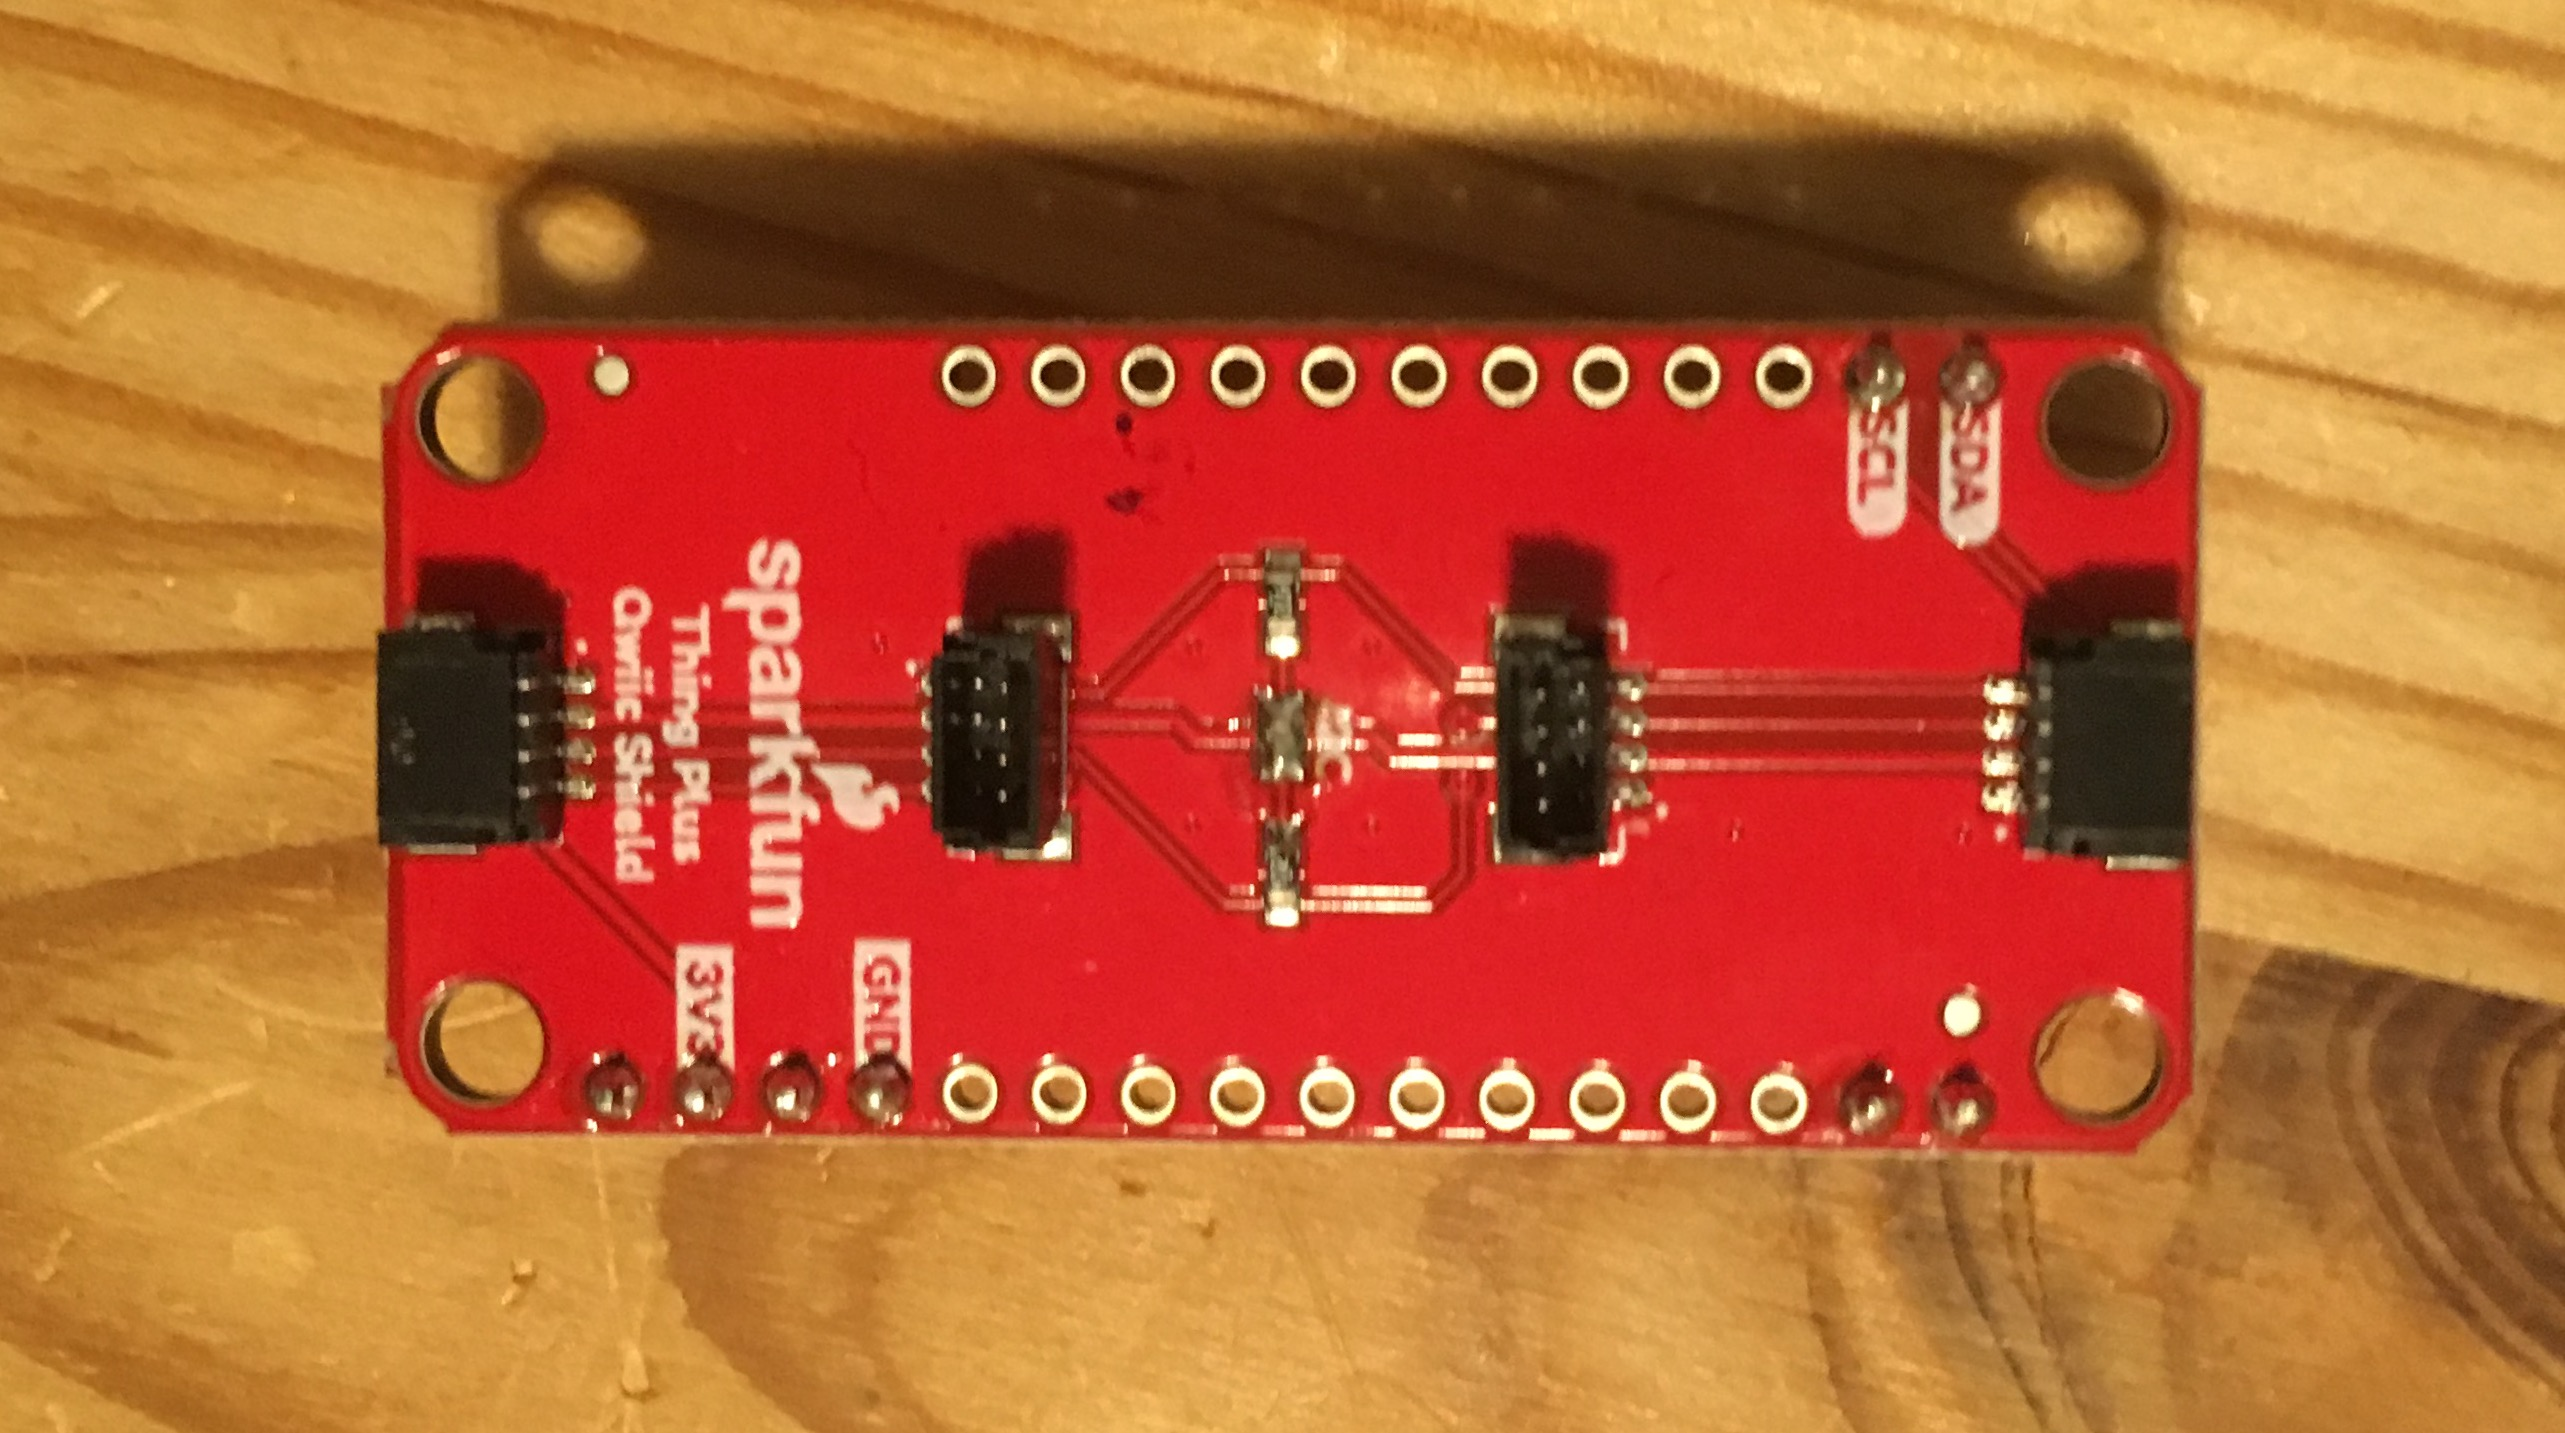
\includegraphics[width=0.45\textwidth]{images/qwiic_top.JPG}
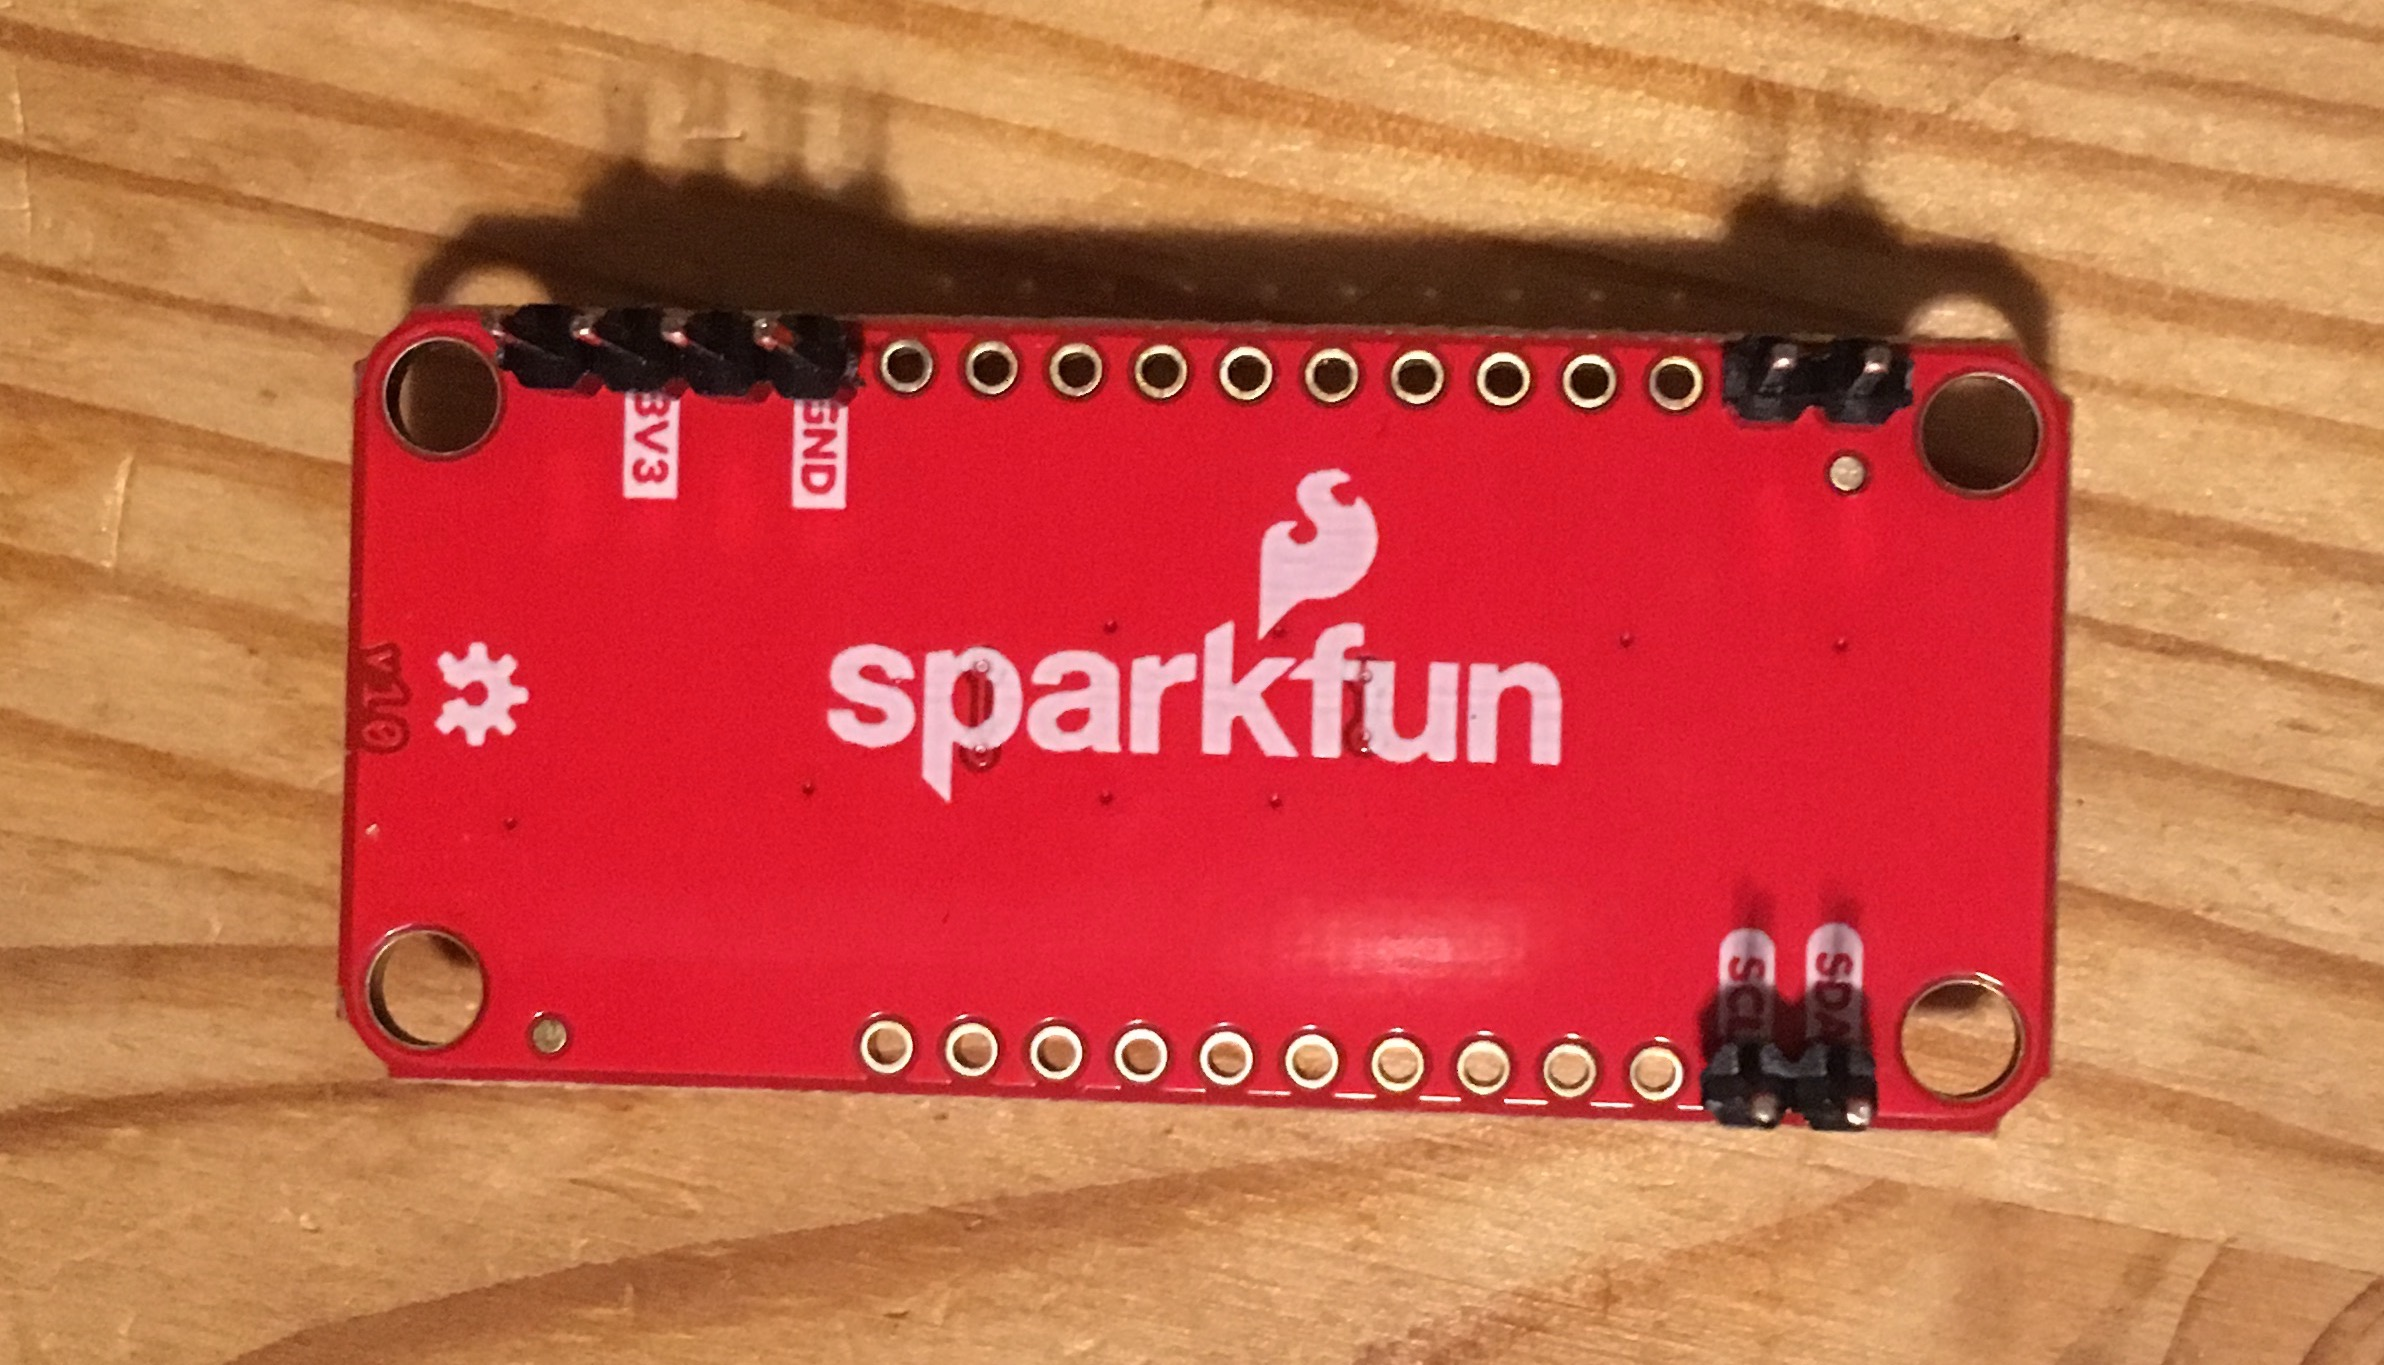
\includegraphics[width=0.44\textwidth]{images/qwiic_bottom.JPG}
\caption{SparkFun Qwiic Shield with male headers and I\textsuperscript{2}C pullups connected} 
\label{fig:qwiic}
\end{figure}

%-----------------------------------------------------------
% ENCLOSURE
\item \label{itm:enclosure}
Enclosure

Before starting this step download and print the drill template. 

\begin{enumerate}[label=2.\arabic*]
\item
Cut out the template and tape it to the enclosure.
\item
Make sure the lid of the enclosure is firmly screwed on before drilling
\item
Drill holes in the locations denoted on template using the recommended drill sizes for each hole. 
\end{enumerate}

%-----------------------------------------------------------
% PRESSURE SENSOR
\item
Pressure Sensor Assembly
\begin{enumerate}[label=3.\arabic*]
\item
Drill out mounting holes refer to figure \ref{fig:bme_1} on page \pageref{fig:bme_1}
\begin{enumerate}[label=3.1.\arabic*]
\item
Using the 7/64'' drill bit, carefully enlarge the mounting holes in each corner of the sensor
\item
You can do all four or just two - one on the left side of one board and one on the right side of the other
\end{enumerate}
\item
Cut trace from SDO through hole to sensor. Refer to figure \ref{fig:bme_1} on page \pageref{fig:bme_1}.
\begin{enumerate}[label=3.2.\arabic*]
\item
Carefully cut the trace coming from the SDO hole on the back side of one board
\item
This board will be used to measure the airway pressure
\end{enumerate}
\begin{figure}[H]
\centering
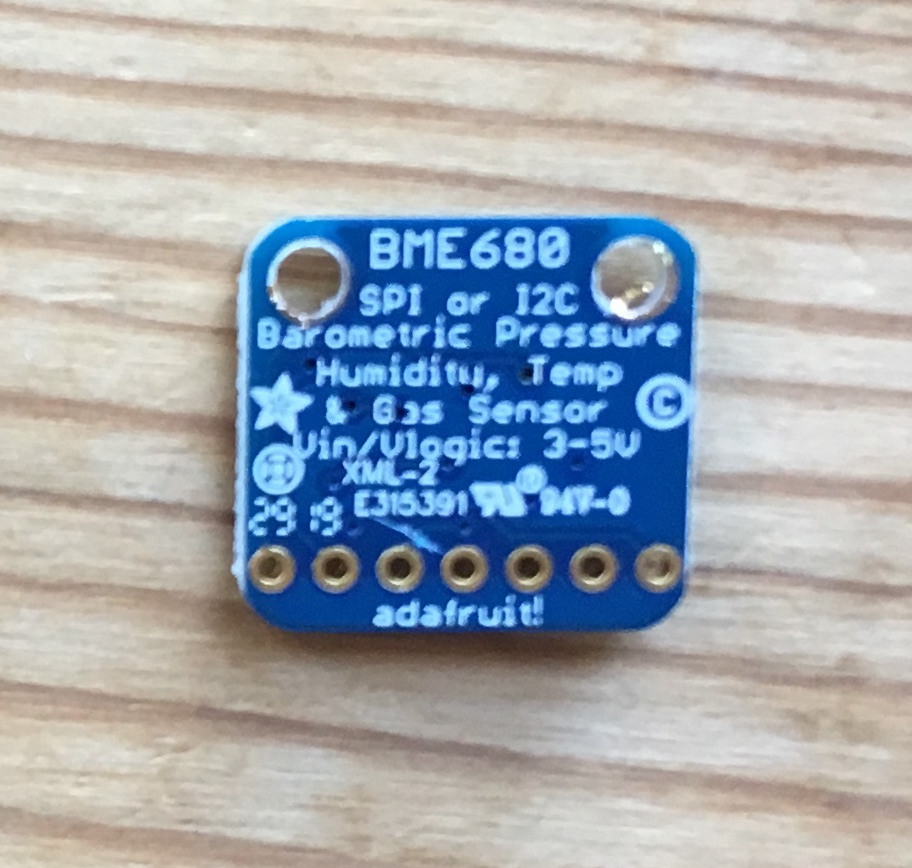
\includegraphics[width=0.45\textwidth]{images/bme_1.JPG}
\caption{BME 280 Eval board with drilled out holes and trace cut} 
\label{fig:bme_1}
\end{figure}

\item
Assemble Cable. Refer to figure \ref{fig:bme_qwiic_cable} on page \pageref{fig:bme_qwiic_cable}.
\begin{enumerate}[label=3.3.\arabic*]
\item
Cut one connector off the Qwiic cable
\item
Strip and tin the last $1/4$" of the leads 
\end{enumerate}
\begin{figure}[H]
\centering
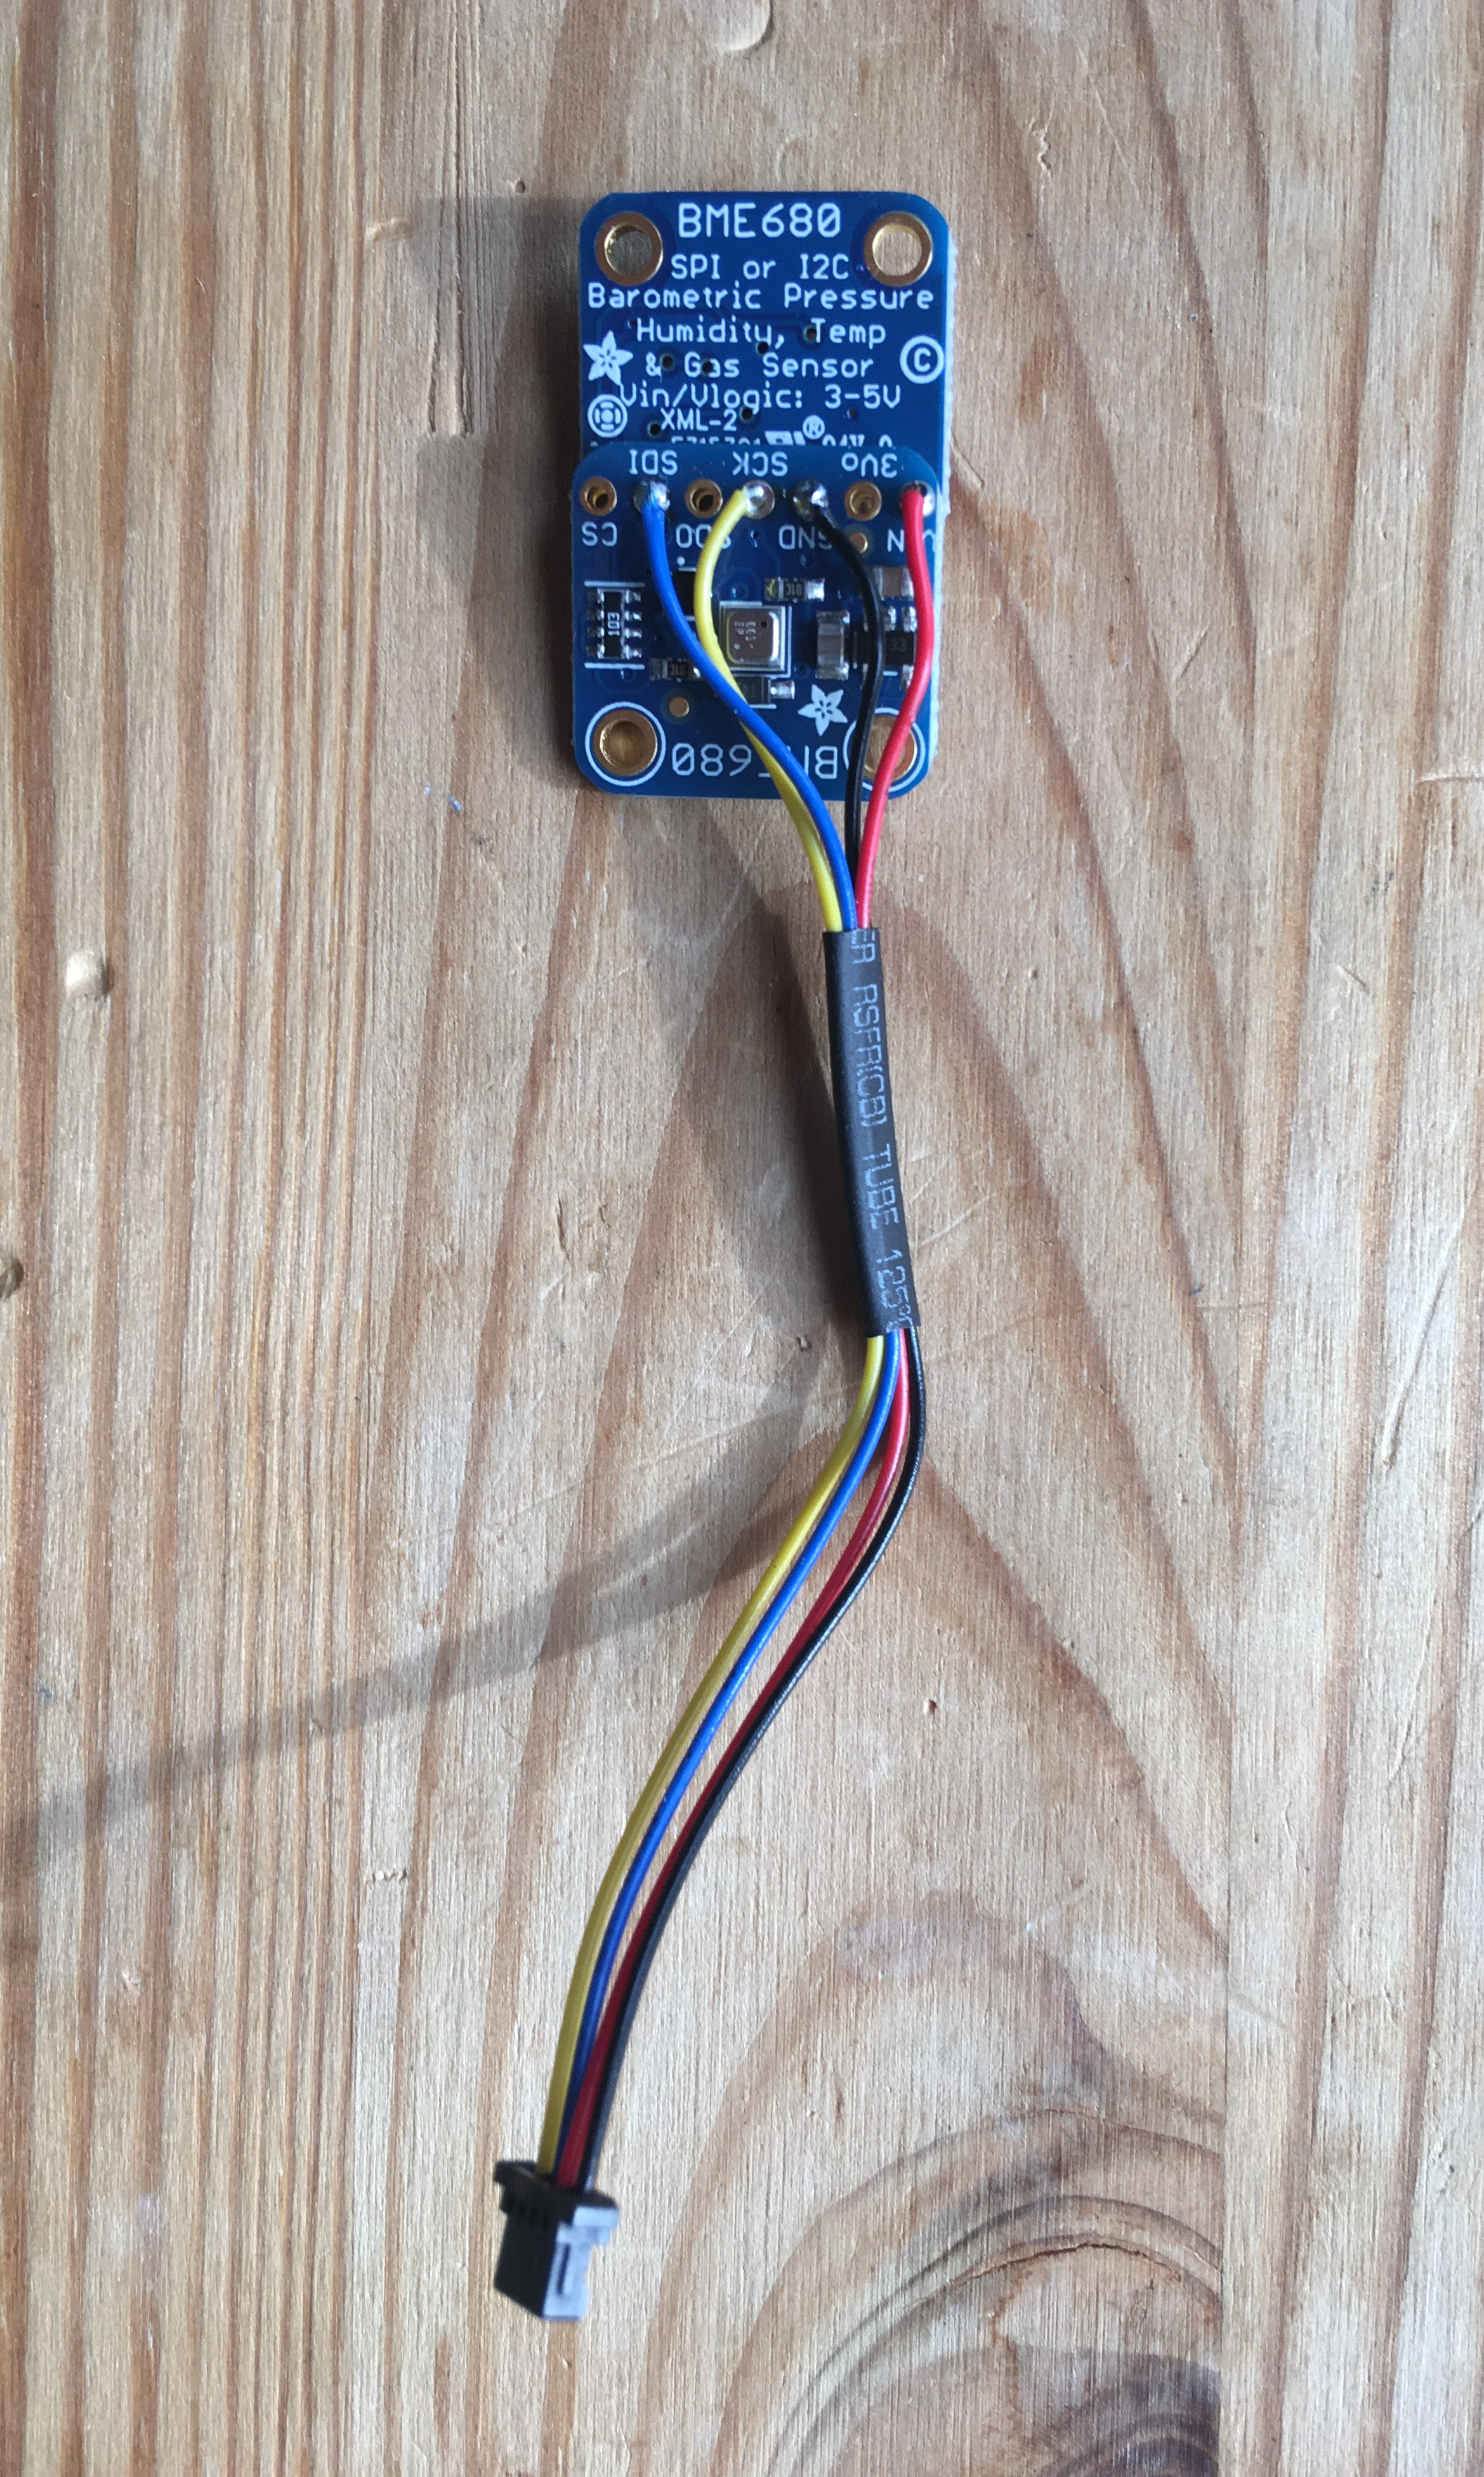
\includegraphics[width=0.5\textwidth]{images/bme_qwiic_cable.JPG}
\caption{Prepared Qwiic cable for BME sensor assembly} 
\label{fig:bme_qwiic_cable}
\end{figure}
\item
Connect Sensors to Cable. Refer to figure \ref{fig:bme_and_qwiic_cable} on page \pageref{fig:bme_and_qwiic_cable} and table \ref{tab:pressure} on page \pageref{tab:pressure} for electrical connection.
\begin{enumerate}[label=3.4.\arabic*]
\item
Stack the two sensors on the breadboard and use two paper clips to anchor them
\item
Be sure the airway board with the cut trace is facing down
\item
Starting with Vin or GND insert the tinned lead through the appropriate hole and apply solder
\item
Flip the sensor assembly over and make sure solder has flowed through both through holes, adding some if needed
\item
Don't worry if the solder does not flow perfectly
\item
Pin the assembly back down and move to another connection following the connection table below
\item
Repeat the steps above until the two boards have been secured and all leads are connected
\item
Re-flow all the joints to ensure a good connection
\end{enumerate}

\begin{table}[H]
\centering
\begin{tabular}{| c | c |}
\hline
Signal & Qwiic Color\\  \hline
GND & black  \\  \hline
VIN & red \\  \hline
SDA & blue \\  \hline
SCL & yellow \\  
\hline
\end{tabular}
\caption{pressure sensor wiring}
\label{tab:pressure}
\end{table}

\begin{figure}[H]
\centering
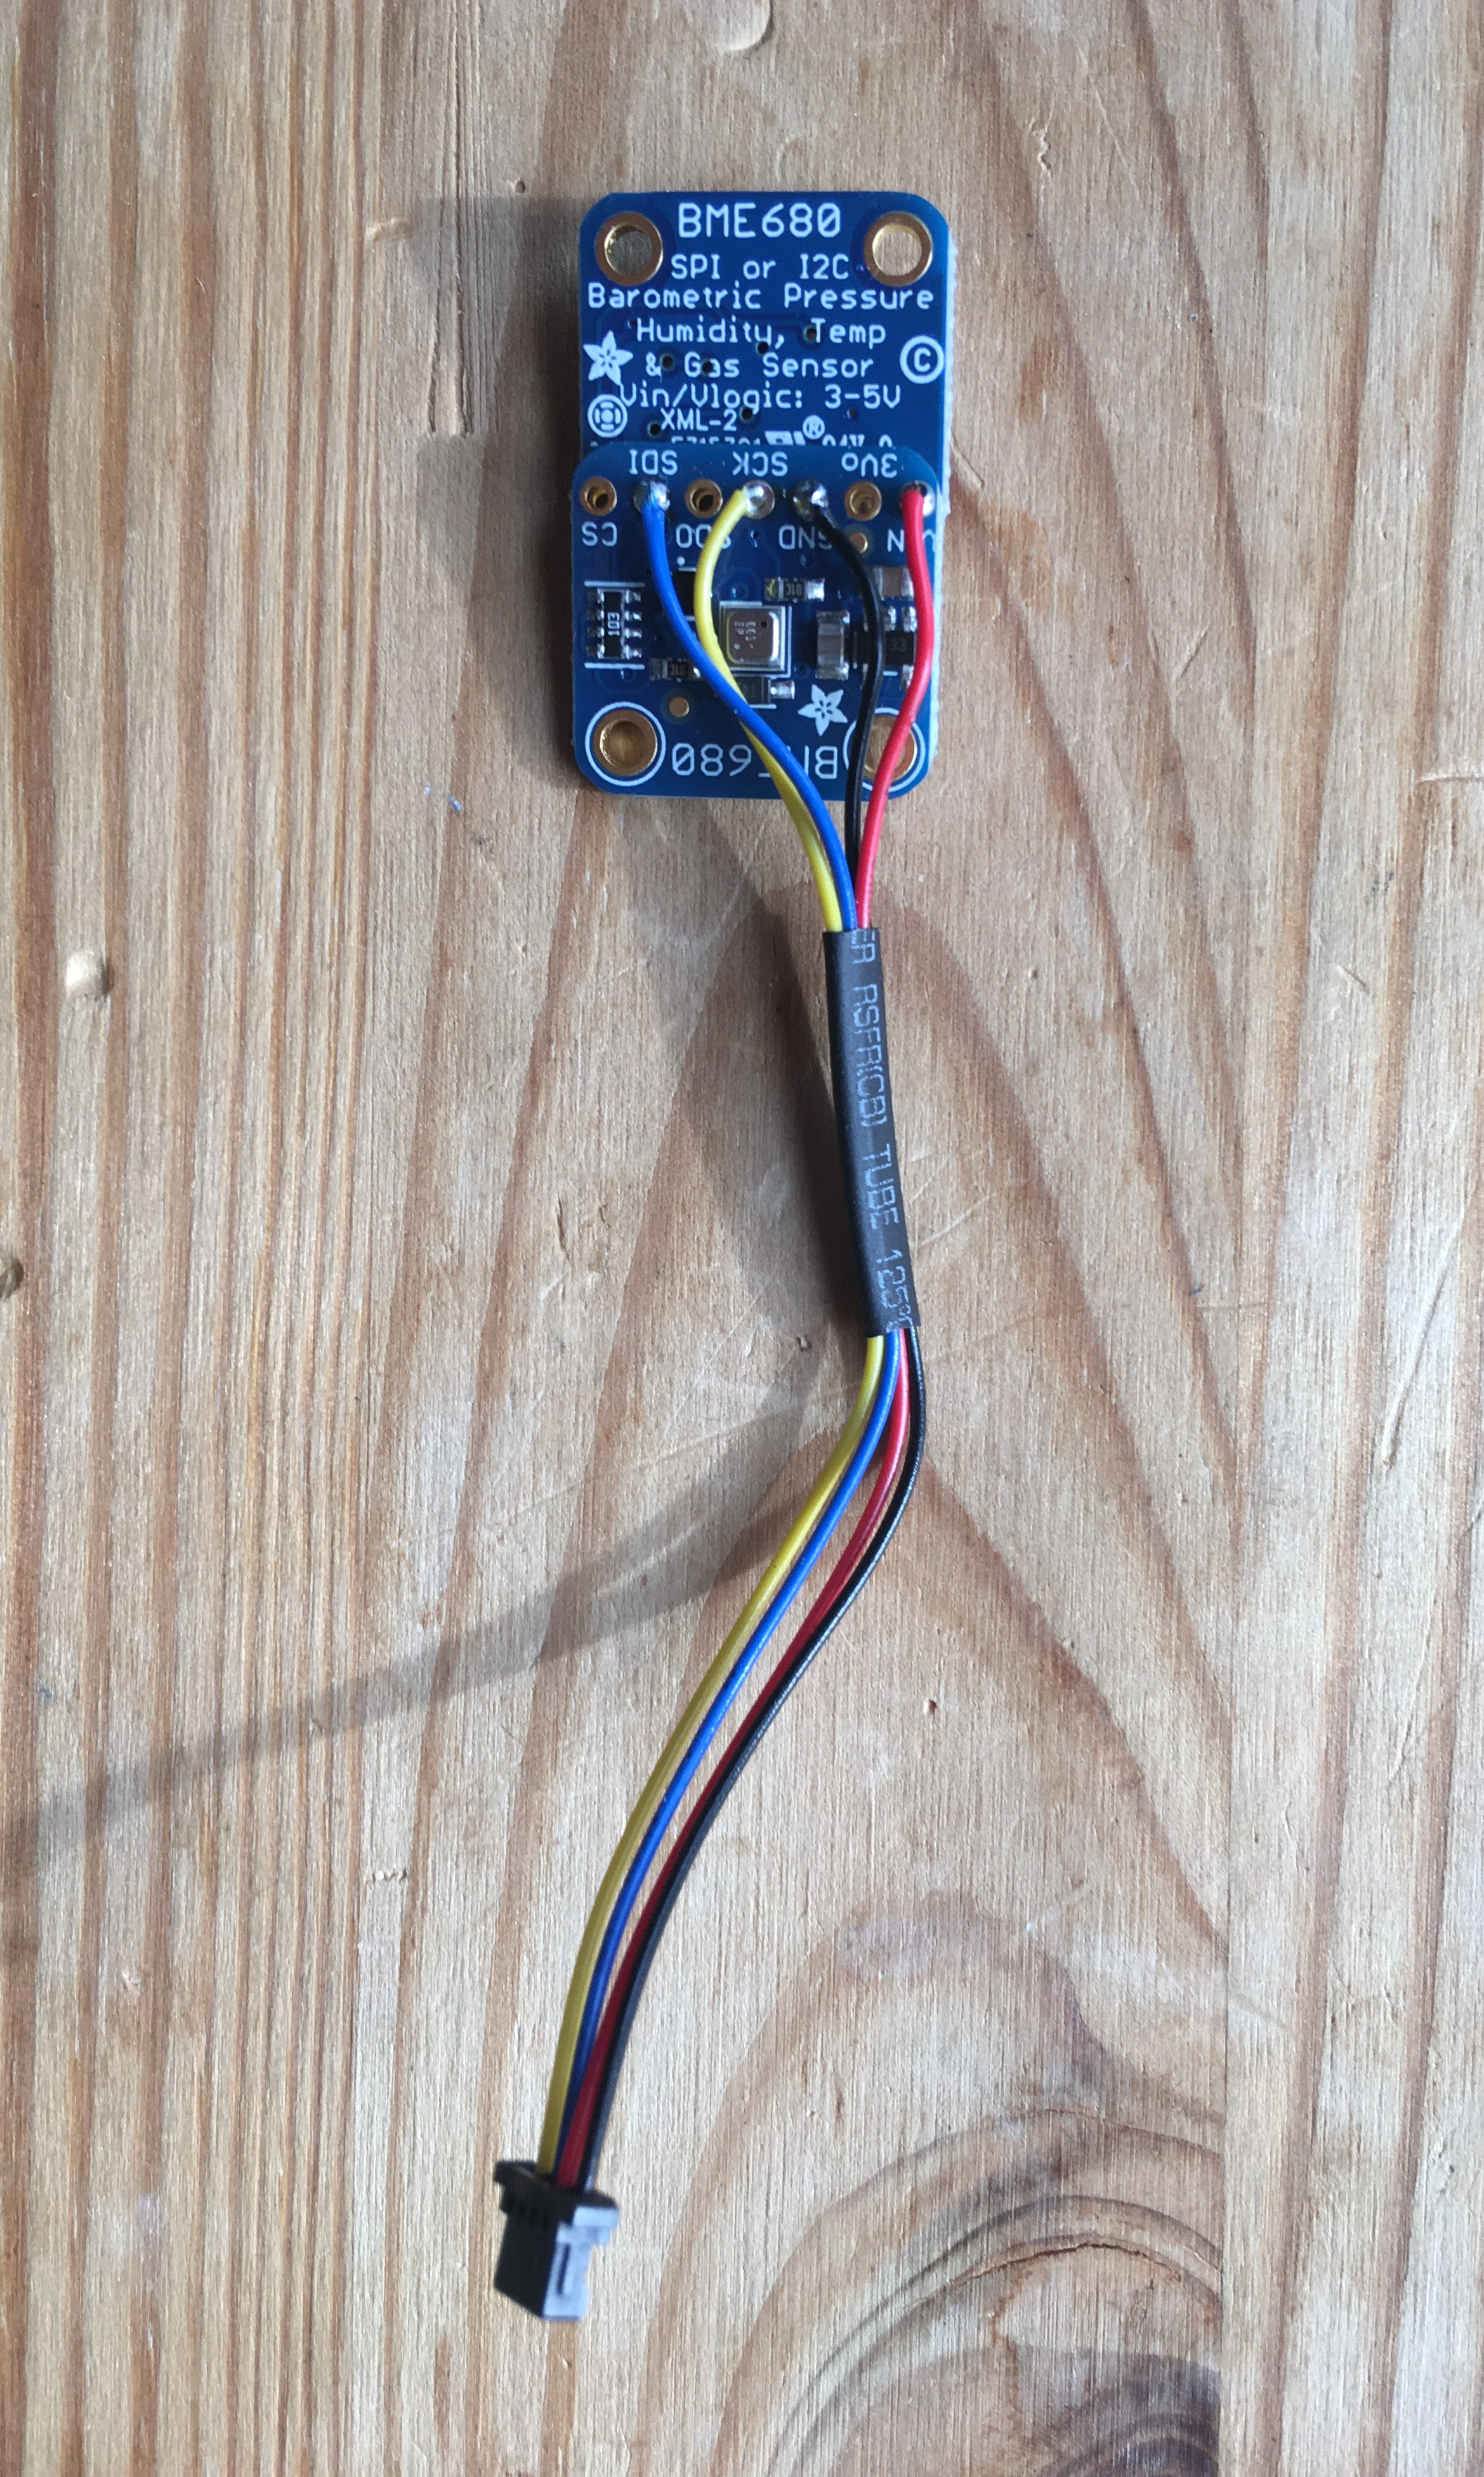
\includegraphics[width=0.65\textwidth]{images/bme_and_qwiic_cable.JPG}
\caption{Qwiic cable soldered to BME sensor assembly} 
\label{fig:bme_and_qwiic_cable}
\end{figure}

\item
Add address jumper to ambient pressure sensor. Refer to figure \ref{fig:bme_diagram} on page \pageref{fig:bme_diagram}
\begin{enumerate}[label=3.5.\arabic*]
\item
Take a $1/2$" piece of hookup wire and strip both ends
\item
Flow the solder in the GND through hole and poke one end of the hook up wire into the hole
\item
Put the other end of the wire into the SDO through hole and apply solder
\end{enumerate}

\begin{figure}[H]
\centering
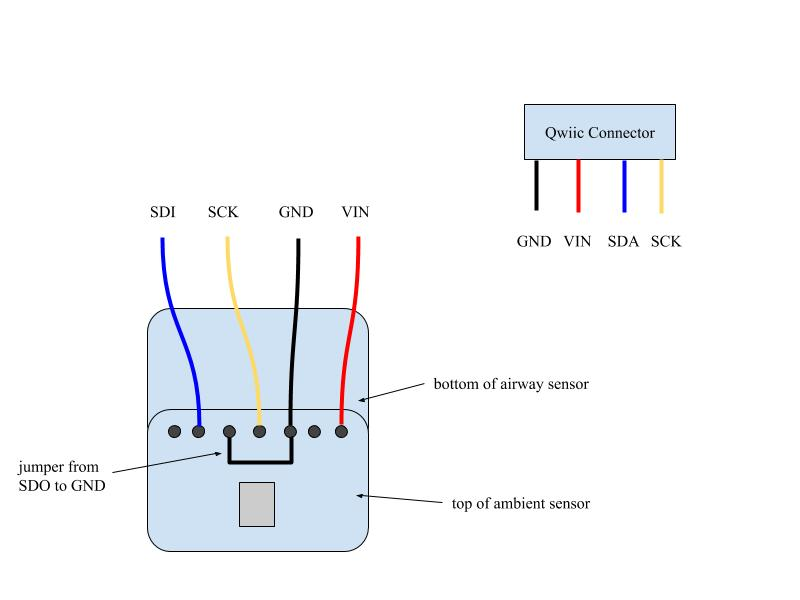
\includegraphics[width=0.75\textwidth]{images/bme_diagram.JPG}
\caption{Qwiic cable soldered to BME sensor assembly} 
\label{fig:bme_diagram}
\end{figure}

\end{enumerate}

%-----------------------------------------------------------
% FLOW SENSOR
\item \label{itm:flow}
Flow Sensor Assembly

\begin{enumerate}[label=4.\arabic*]
\item
Assemble Cable. Refer to figure \ref{fig:flow_cable} on page \pageref{fig:flow_cable}

The flow sensor requires a 5 V input, however we will run the I$^2$C bus at 3.3 V necessitating this cable. 
\\
\begin{enumerate}[label=4.1.\arabic*]
\item
Cut the Qwiic cable in half
\item
Cut off the red conductor near the base of the connector
\item
Cut a 30 cm length from the USB cable
\item
Strip the jacket back 1 $1/2$'' from one end
\item
Strip the first $1/4$'' of each conductor on one end and tin
\item
Twist a small portion of the shield into the black GND conductor
\item
Place a small piece of heat shrink on each conductor of the Qwicc cable and push them toward the connector end
\item
Solder the ends of the Qwiic cable to the ends of the USB cable following Table \ref{tab:flow}.
\begin{table}[H]
\centering
\begin{tabular}{| c | c | c |}
\hline
USB & Qwiic & Signal \\  \hline
black & black & GND \\  \hline
green & blue & SDA \\  \hline
white & yellow & SCK \\  \hline
red & single 6'' wire & 5V \\  
\hline
\end{tabular}
\caption{flow sensor wiring}
\label{tab:flow}
\end{table}
\item
Connect the red wire to the red conductor in the USB cable and solder the extra long male header pin to the end
\item
Cover the finished joints with a short $1/4$'' piece of heat shrink
\end{enumerate}

\begin{figure}[H]
\centering
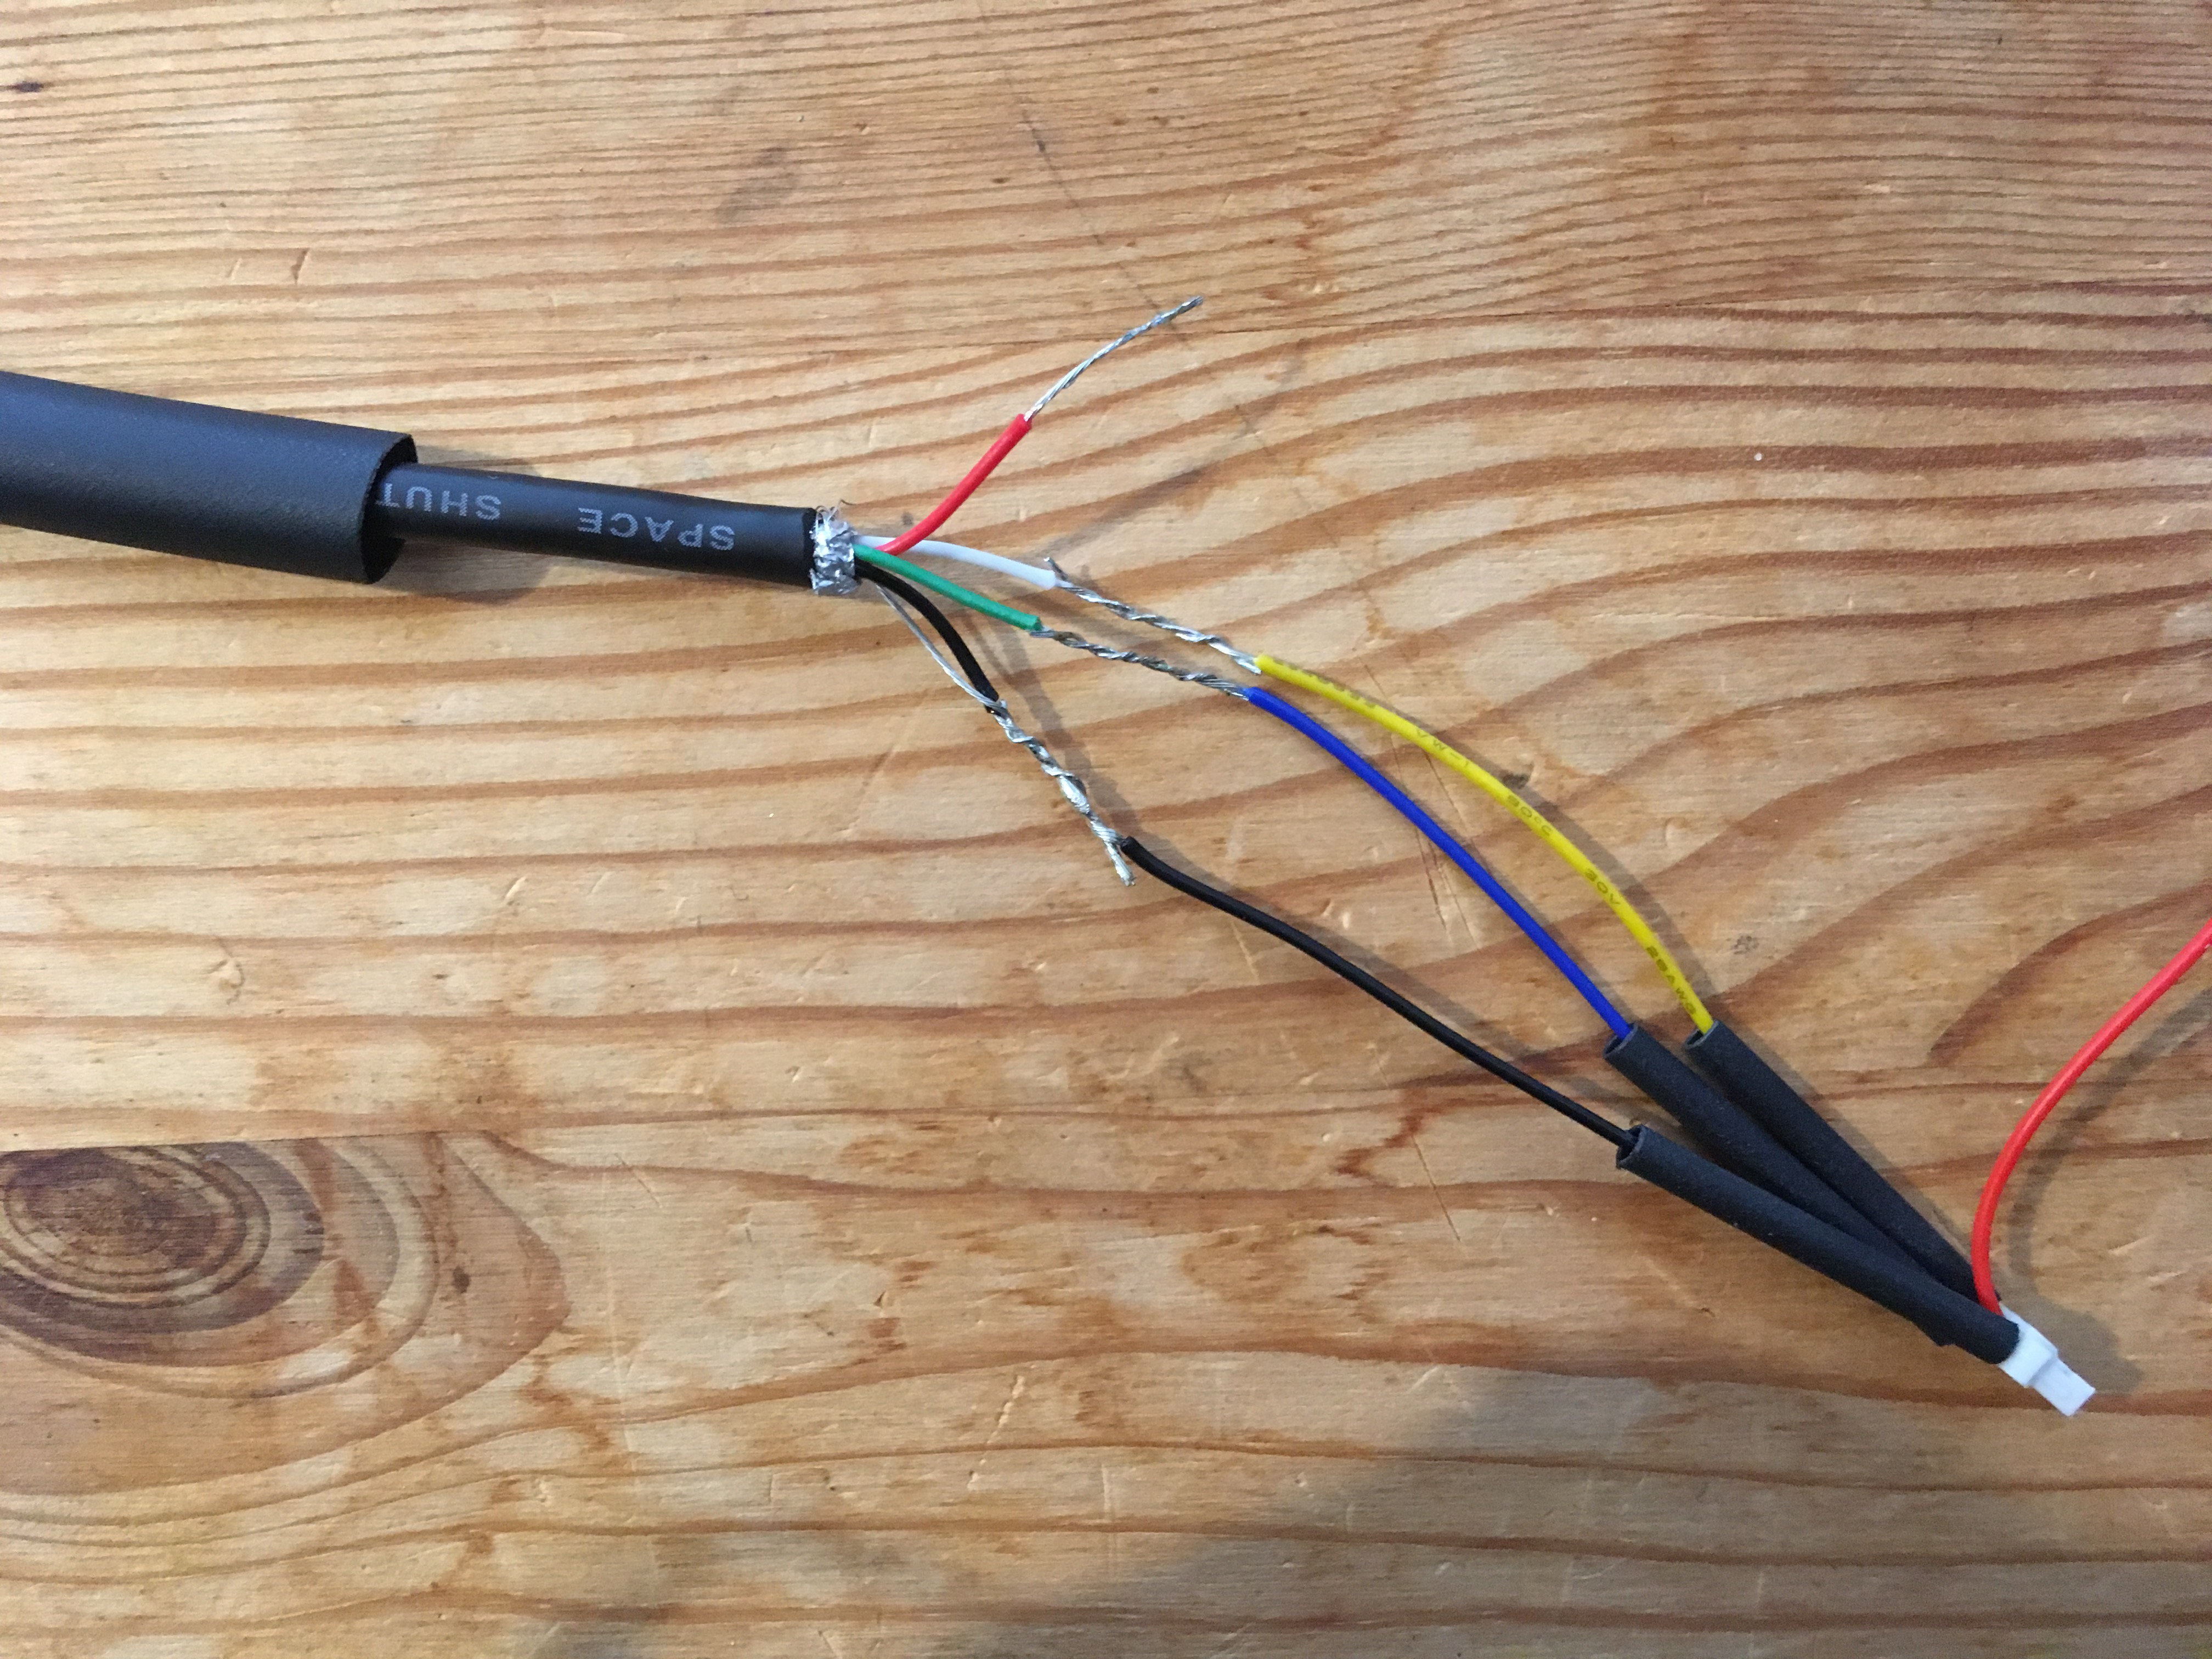
\includegraphics[width=0.45\textwidth]{images/flow_1.JPG} 
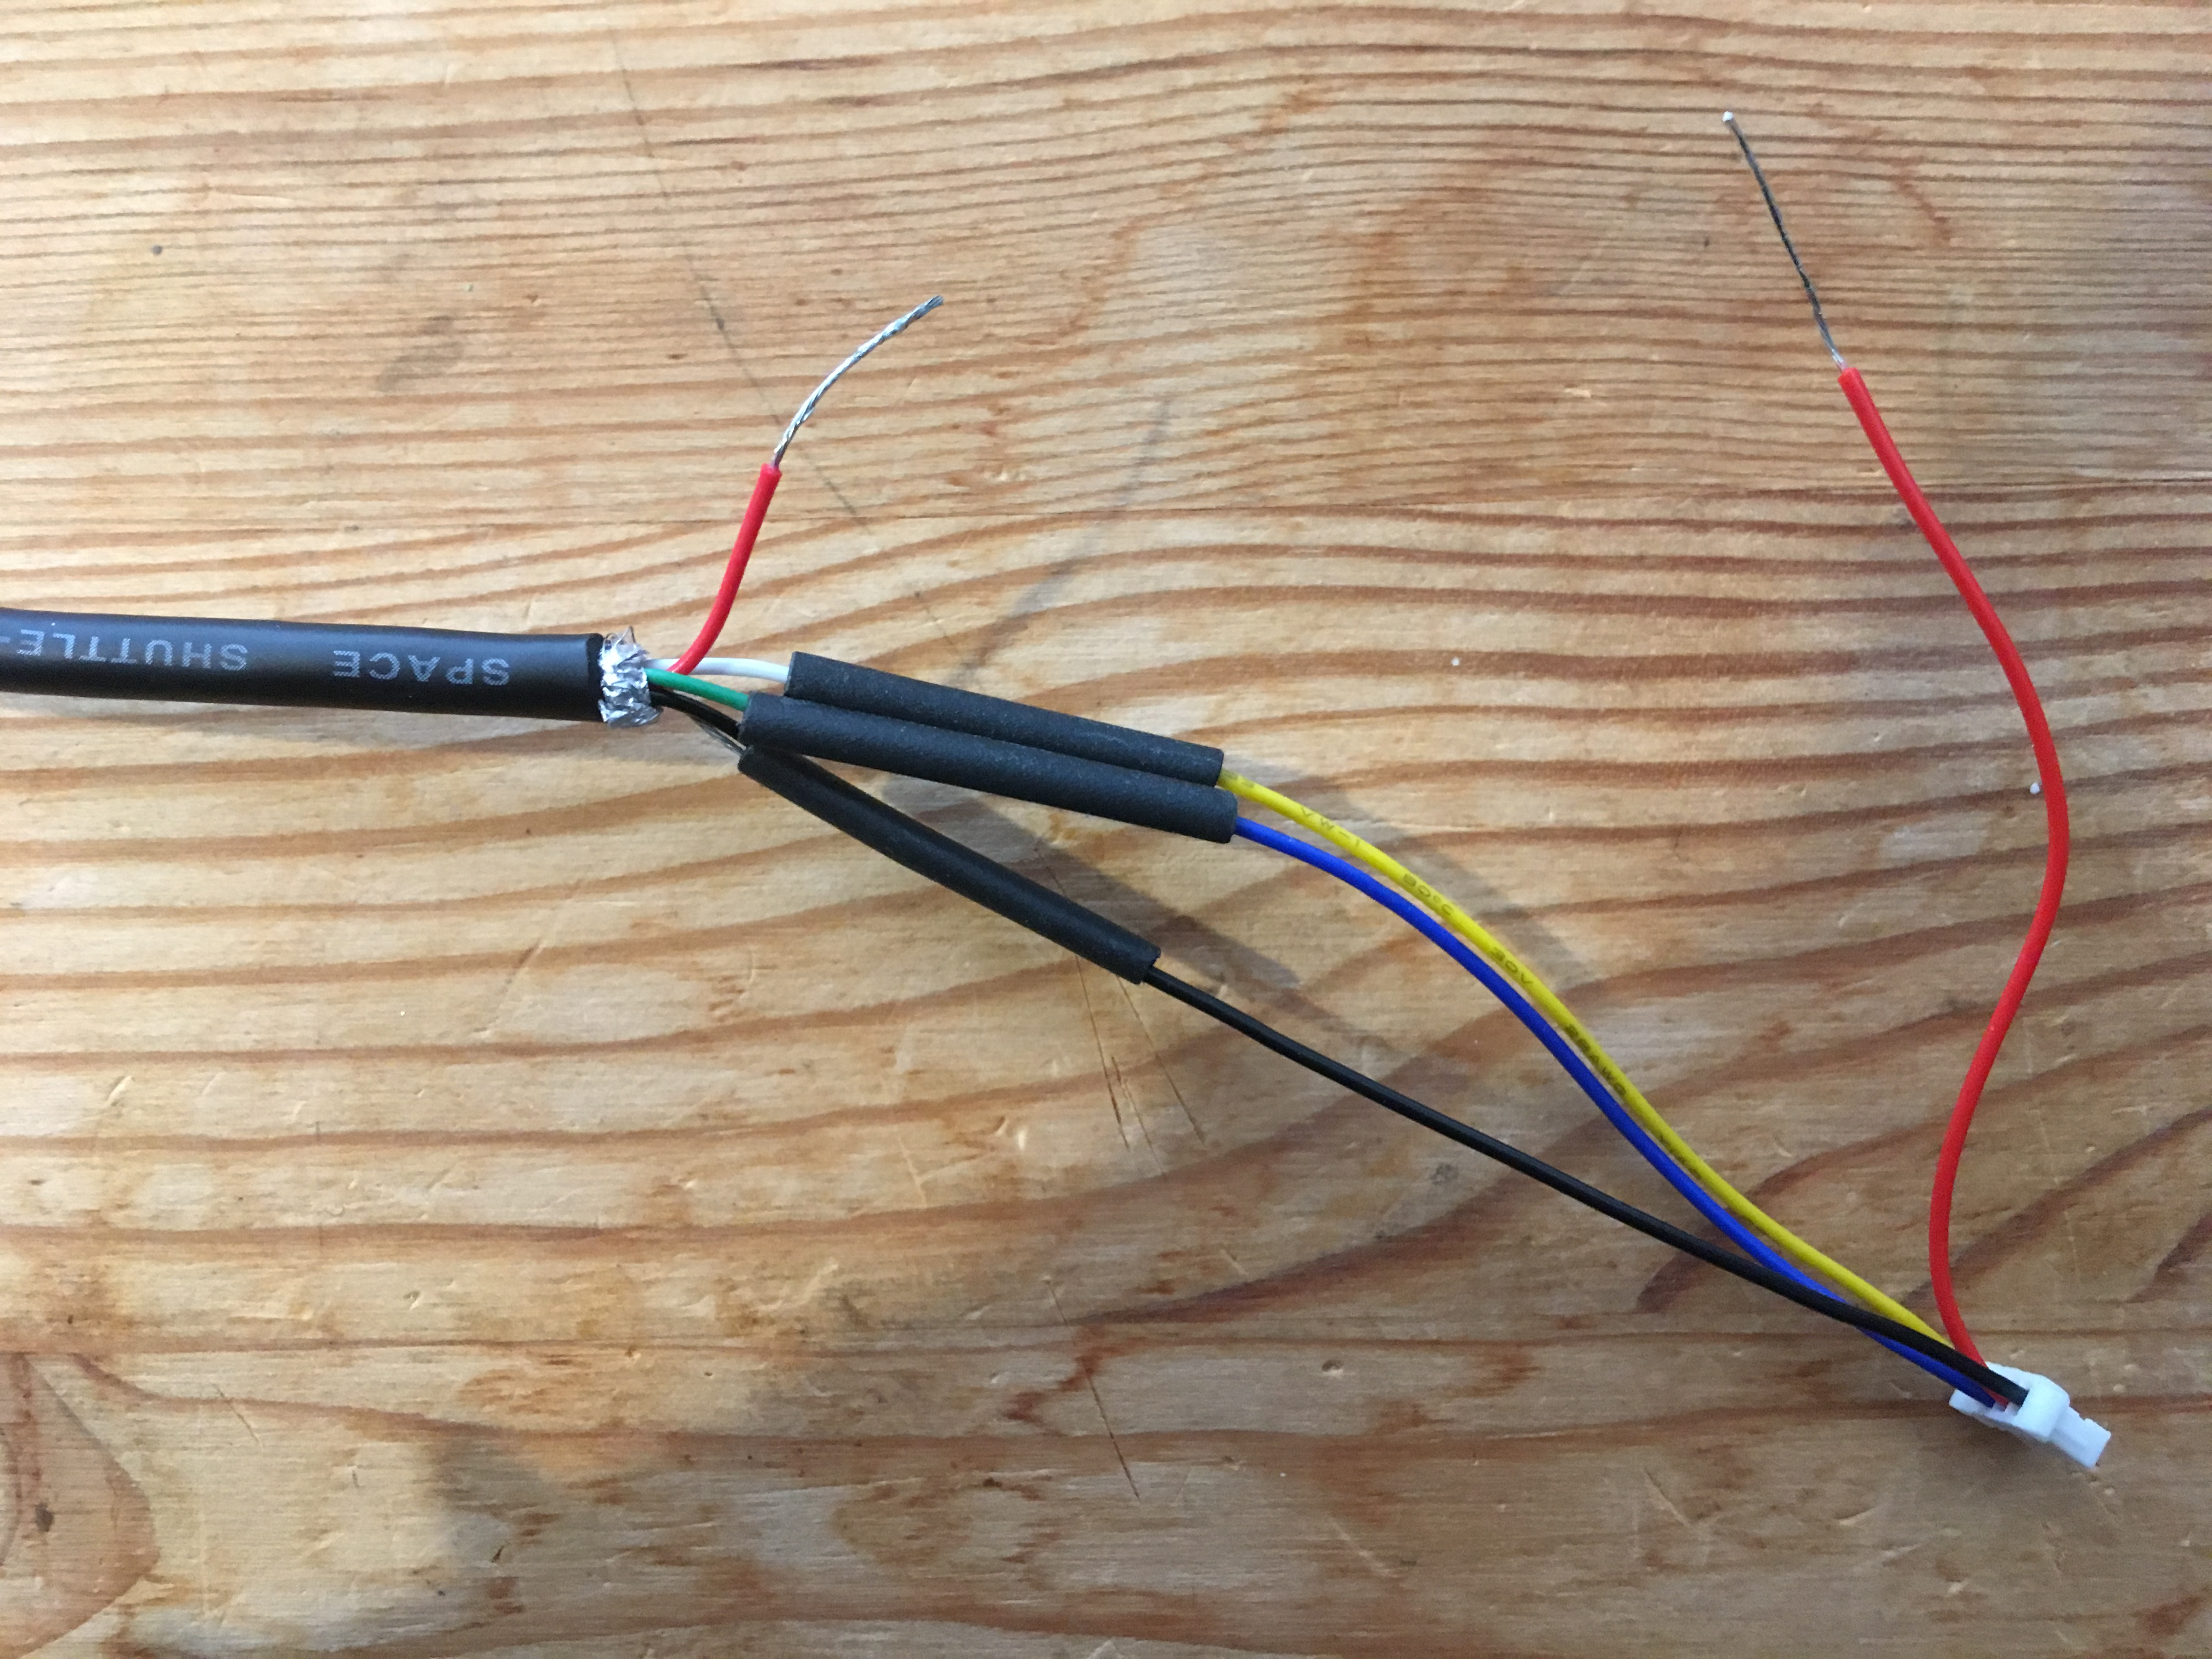
\includegraphics[width=0.45\textwidth]{images/flow_2.JPG} \\ 
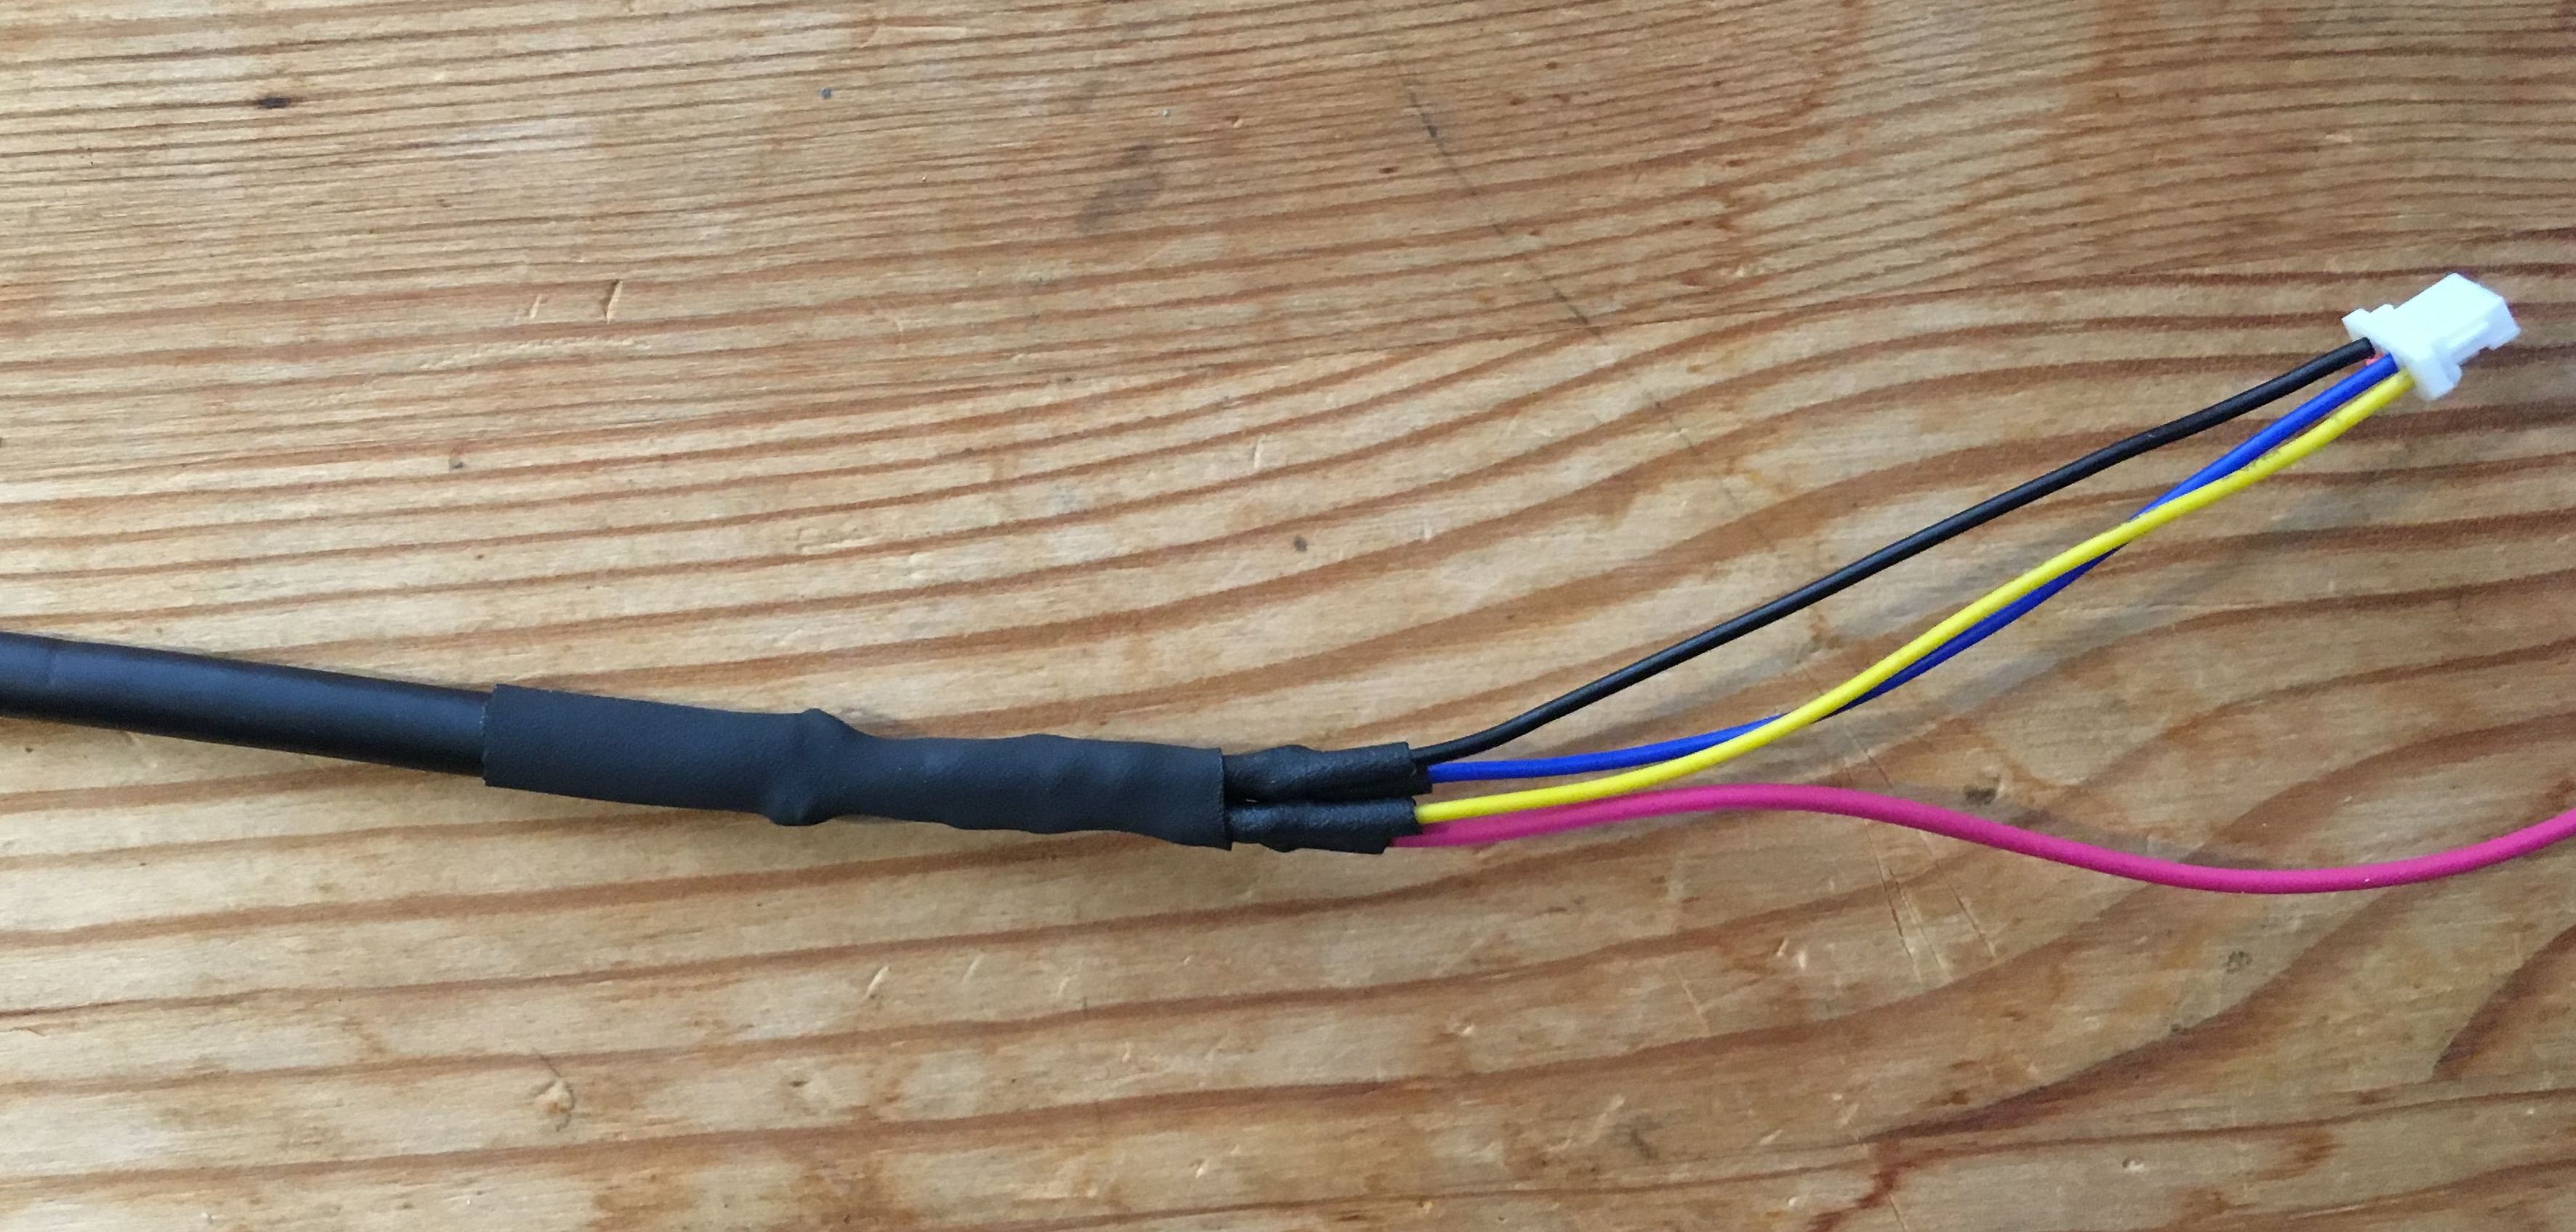
\includegraphics[width=0.45\textwidth]{images/flow_4.JPG} 
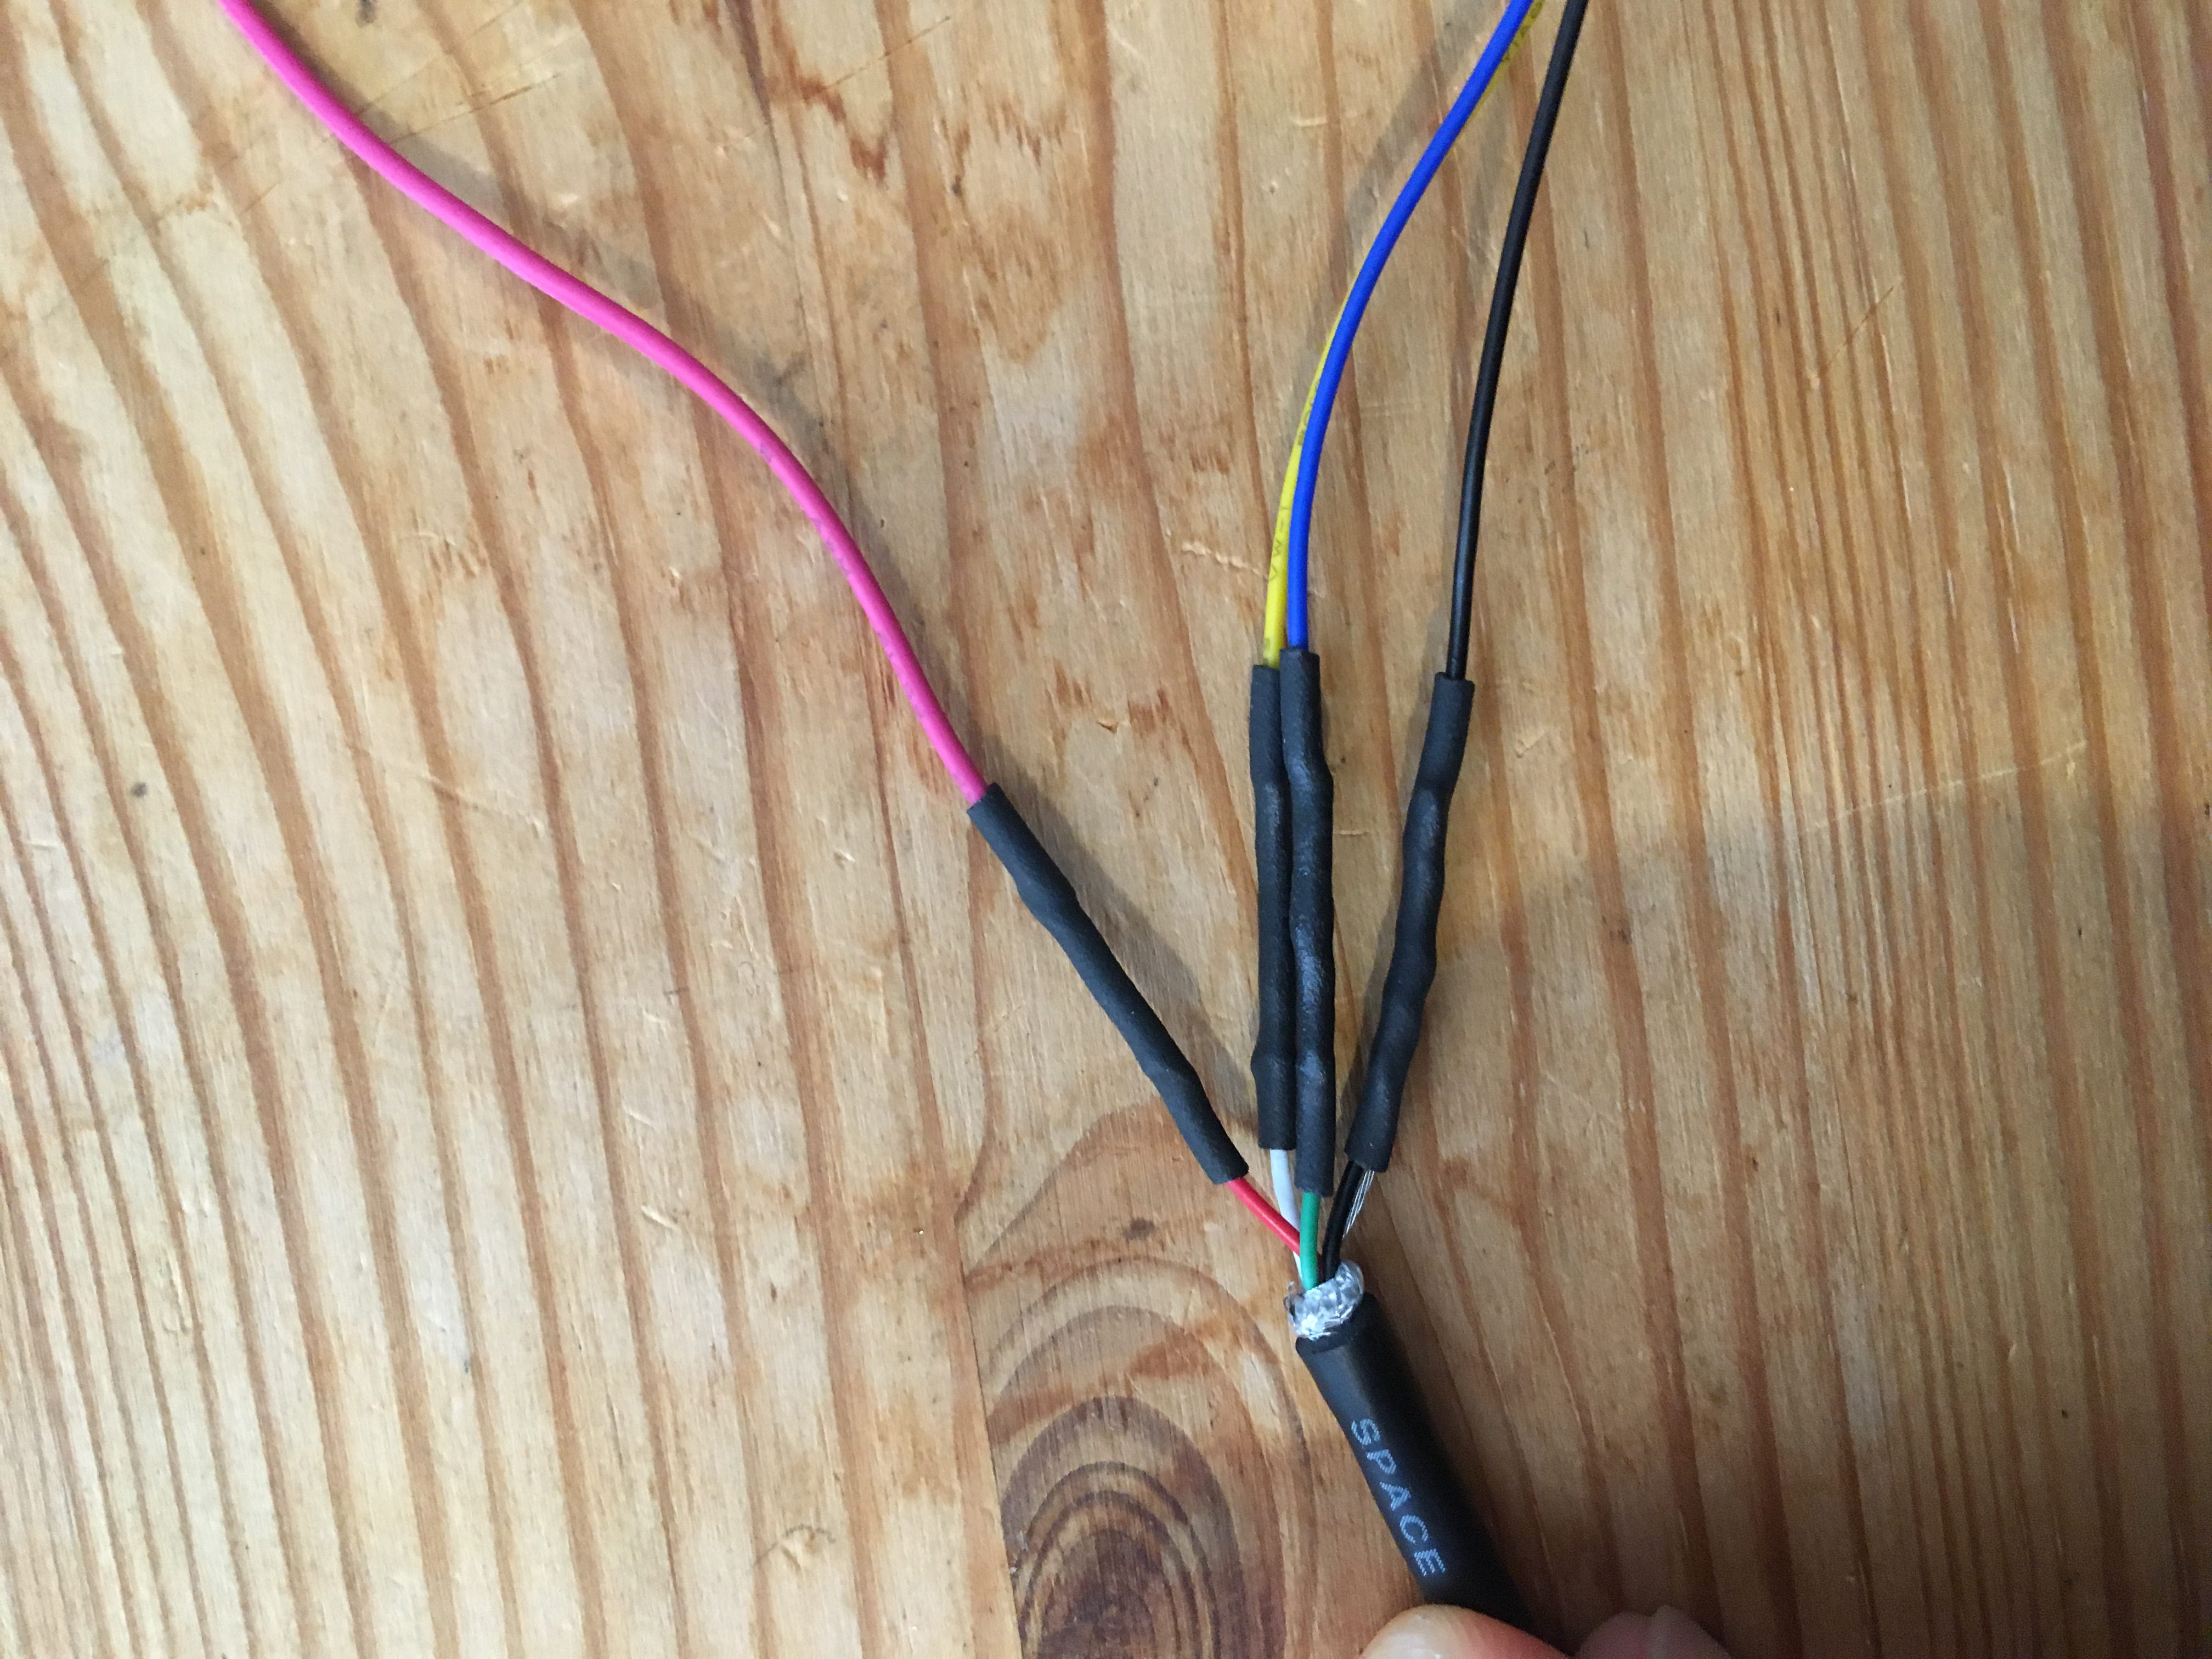
\includegraphics[width=0.45\textwidth]{images/flow_3.JPG} 
\caption{Clockwise progression of sensor cable assembly.} 
\label{fig:flow_cable}
\end{figure}

\item
Connect cable to sensor.  Refer to figure \ref{fig:flow_sensor} on page \pageref{fig:flow_sensor}.

\begin{enumerate}[label=4.2.\arabic*]
\item
Apply a small quantity of solder to the four center pads on the SFM3400 flow sensor
\item
Remove $5/8$'' of the jacket on the bare end of the USB cable
\item
Strip back $1/8$'' from each conductor and tin the ends
\item
Thread the cable through the hole in the sensor as shown in the photo and make sure the tinned leads can reach the sensor pads
\item
Connect the end of each lead to the pads you have prepared by touching the tip of the soldering iron to the pad and then placing the tinned lead onto it.
\item
Refer to the SFM3400 datasheet to be sure you are connecting them in the proper position.
\end{enumerate}
\begin{figure}[H]
\centering
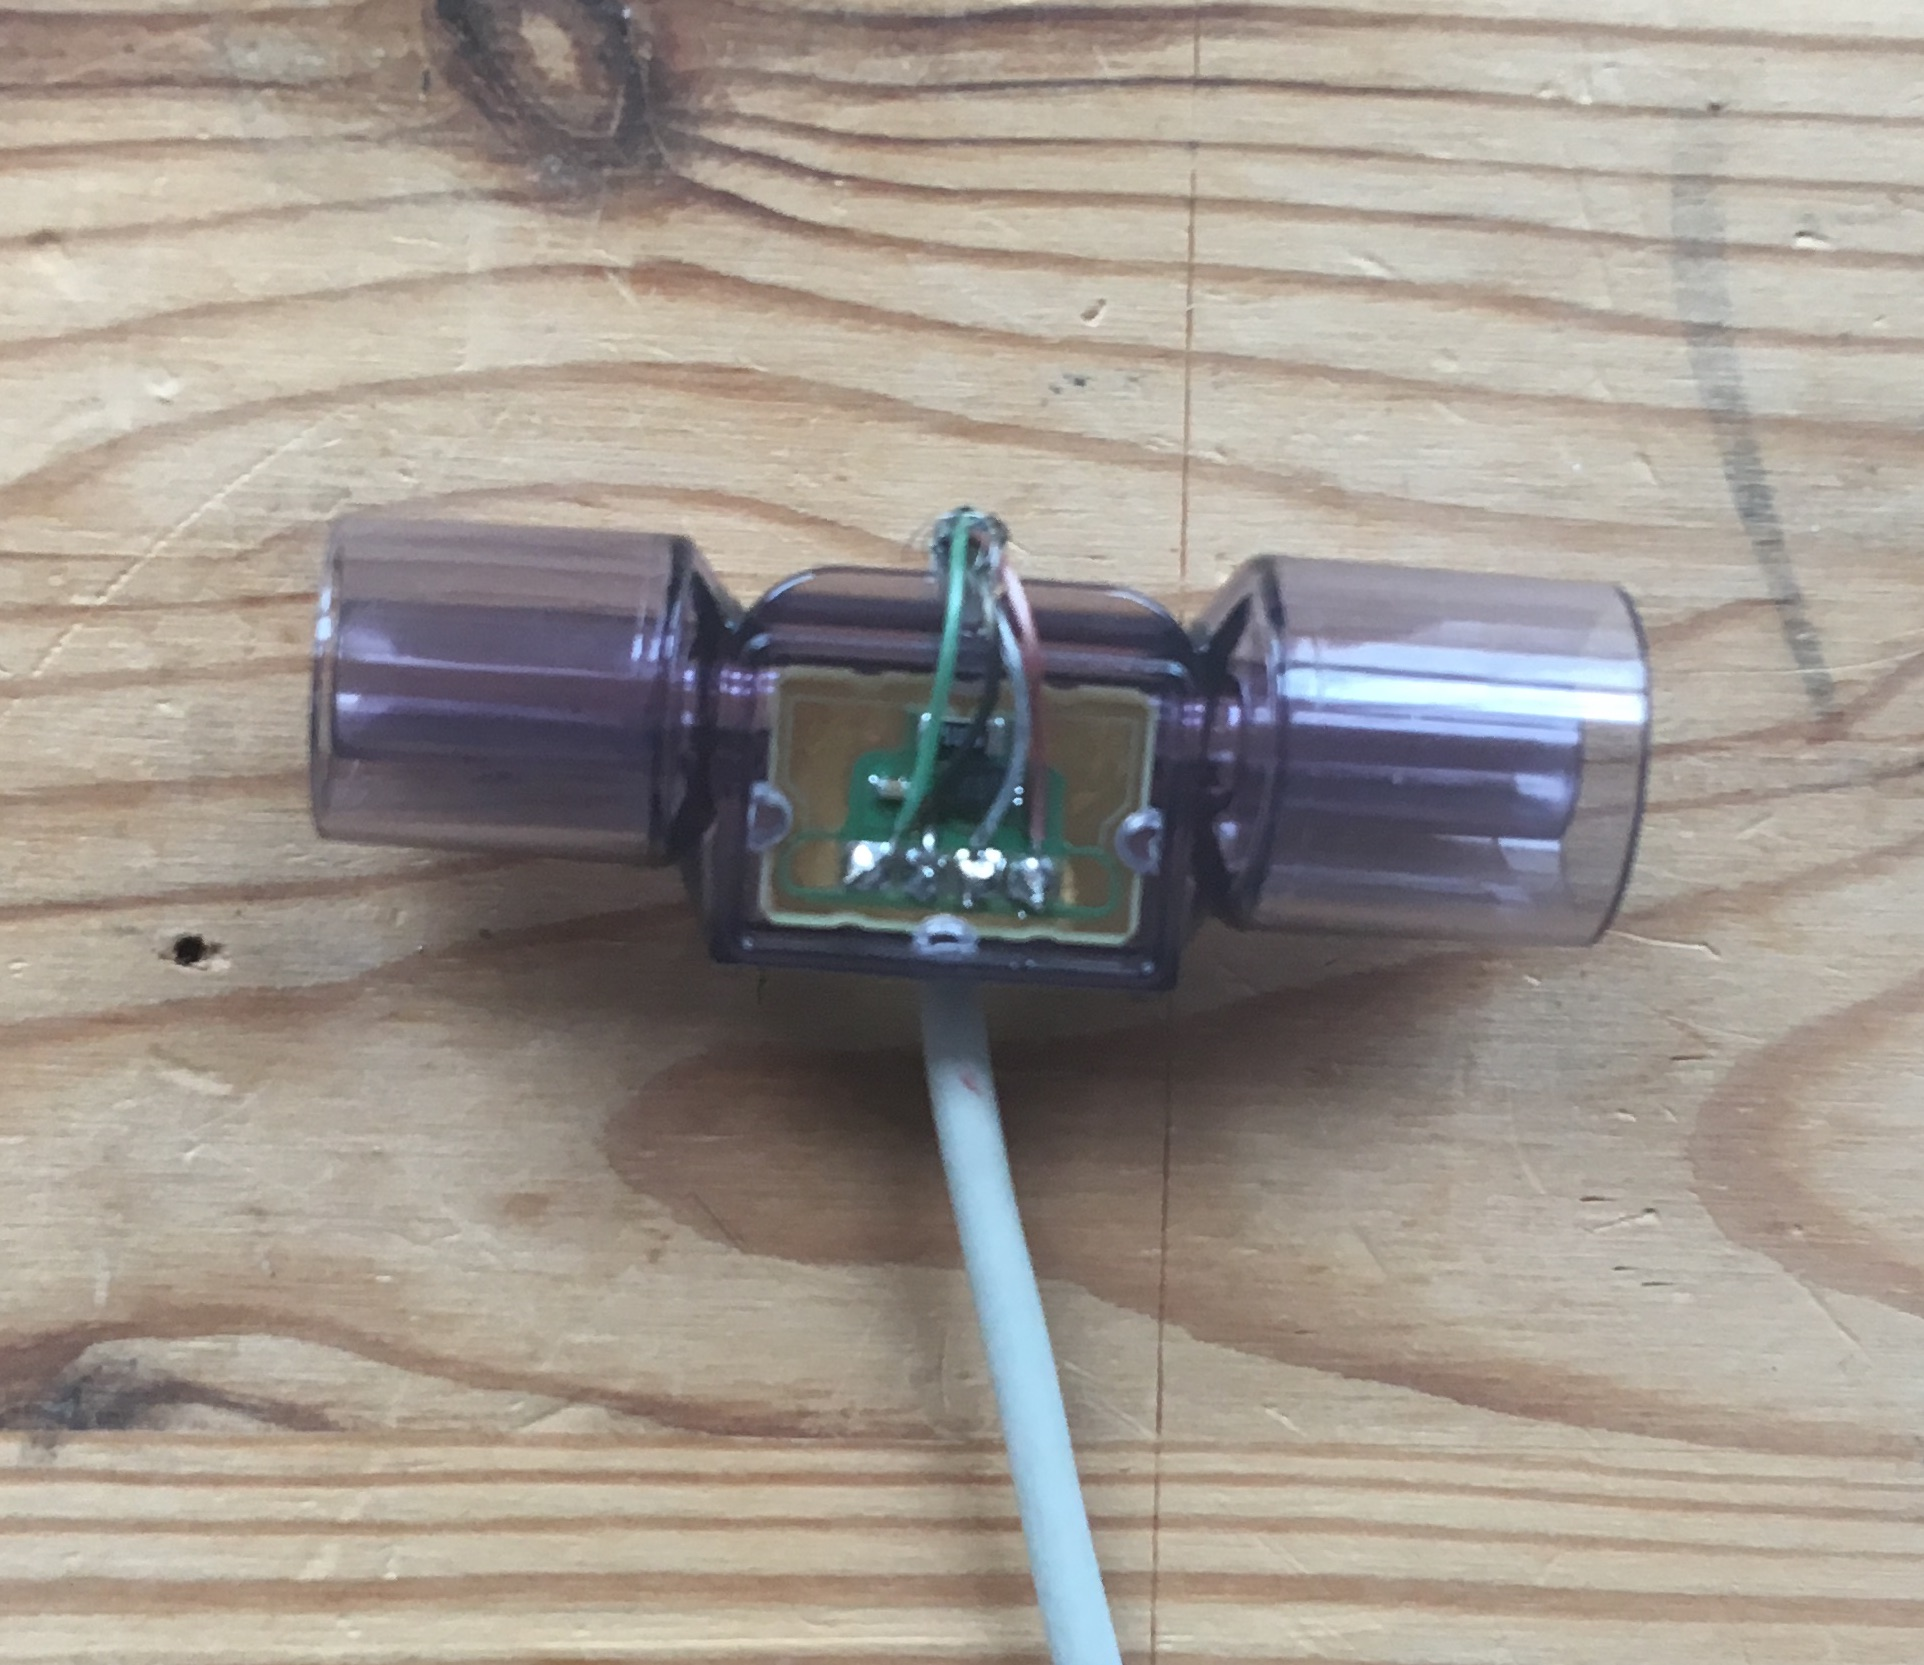
\includegraphics[width=0.6\textwidth]{images/flow_cable.JPG} 
\caption{Sensor connected to cable assembly.} 
\label{fig:flow_sesor}
\end{figure}

\item
Assemble sensor adapters. Refer to figure \ref{fig:adapters} on page \pageref{fig:adapters}.

\begin{enumerate}[label=4.3.\arabic*]
\item
Cut a 1 $1/2$'' section of petex tubing
\item
Insert the tubing into the wide end of the flow sensor
\item
Insert the frosted 15 mm to 22 mm adapter over the petex
\item
Add the clear 15 mm to 22 mm adapter over the small end of the flow sensor
\item
Place the bleed adapter over the clear adapter
\item
Use electrical tape to secure any loose connections
\end{enumerate}
\begin{figure}[H]
\centering
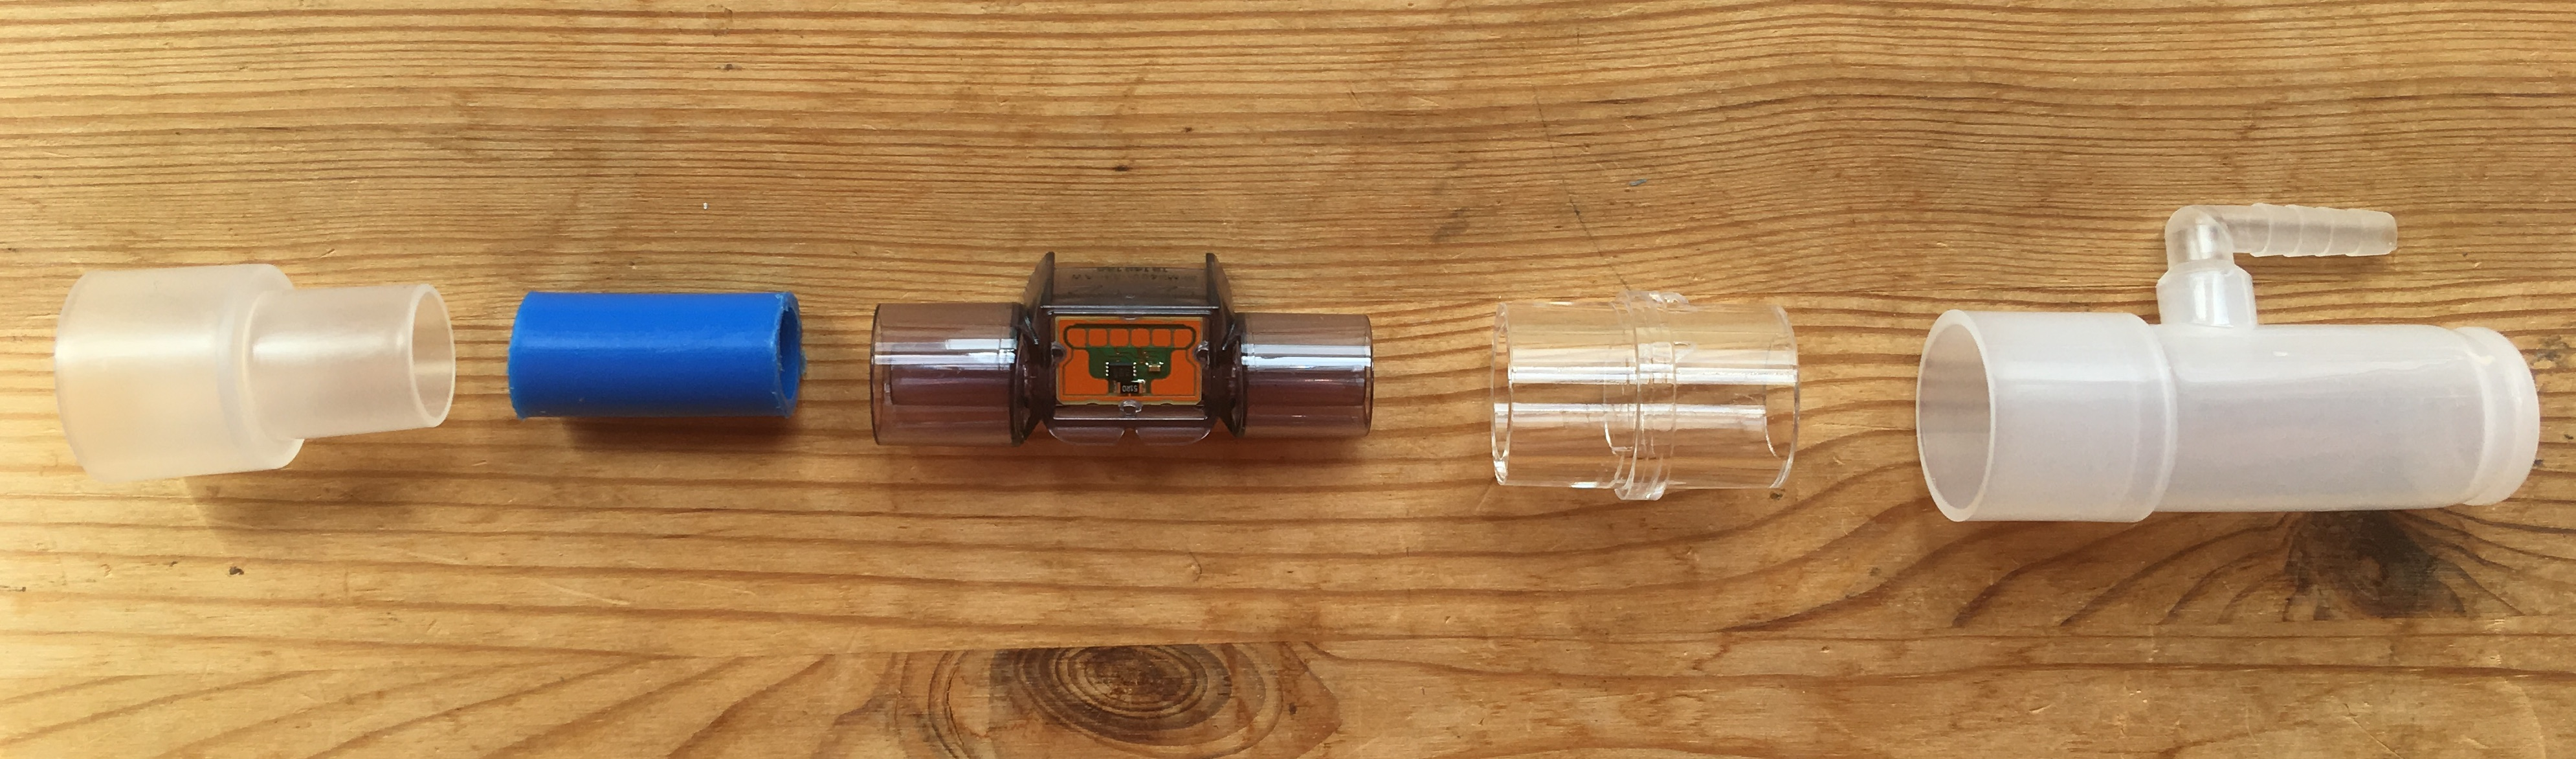
\includegraphics[width=0.8\textwidth]{images/adapters_1.JPG} \\
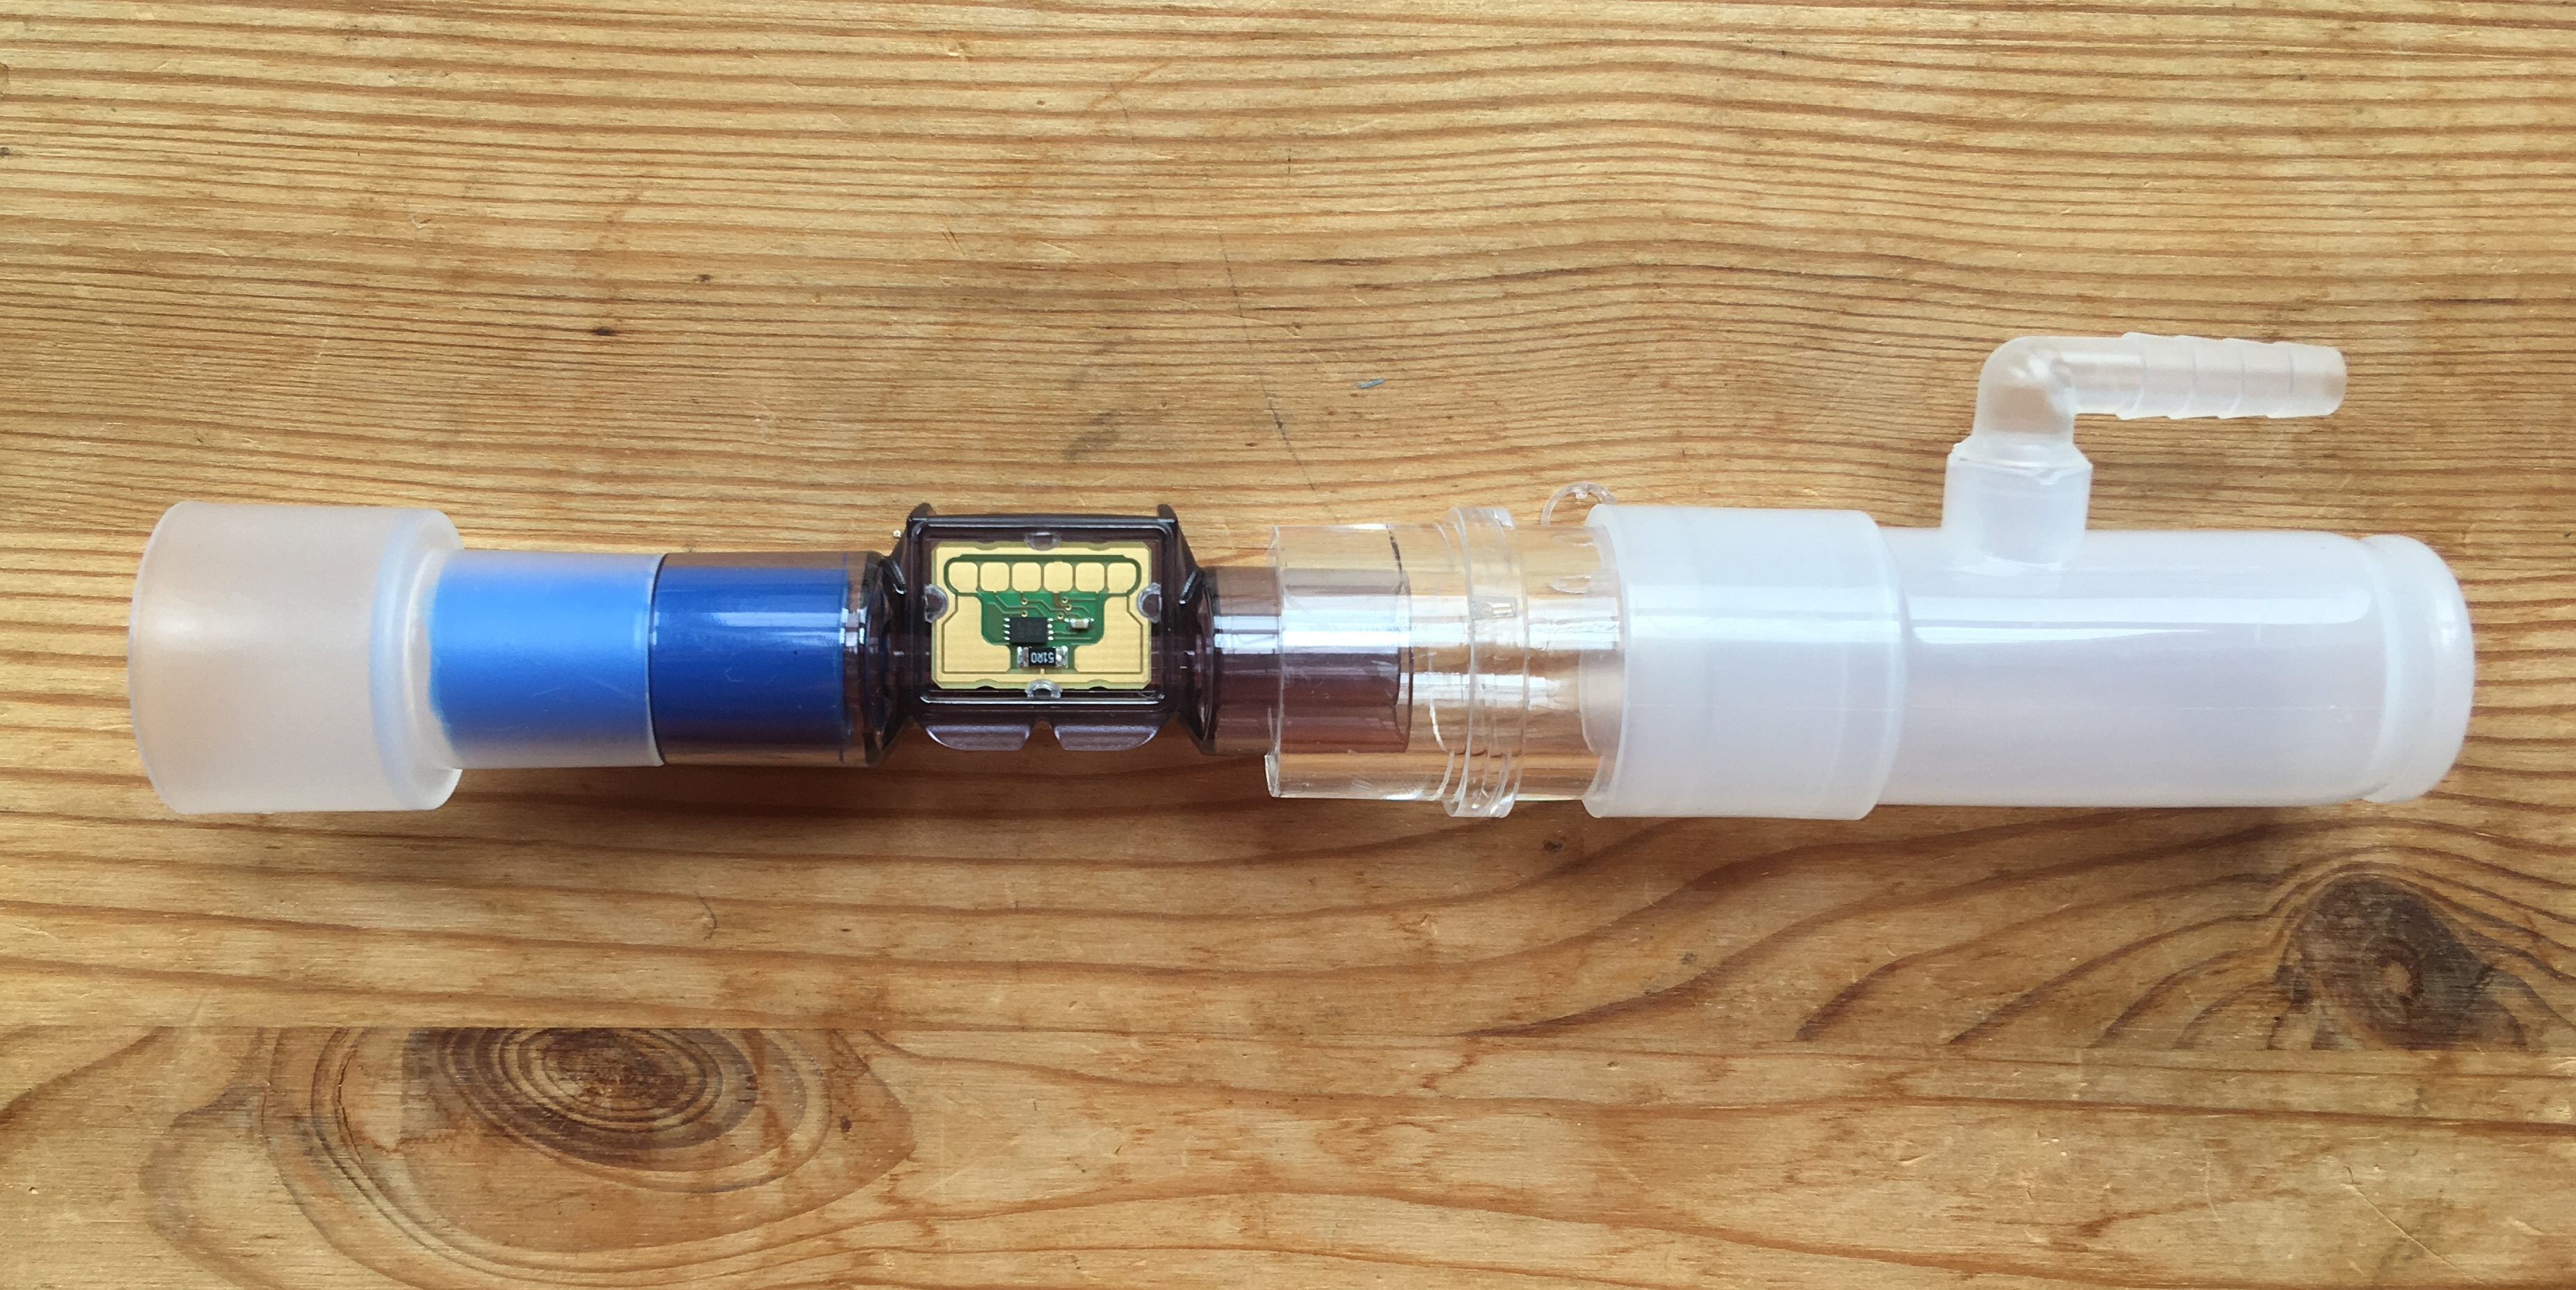
\includegraphics[width=0.6\textwidth]{images/adapters_2.JPG} \\
\caption{Adapters assembled inline with sensor.} 
\label{fig:adapters}
\end{figure}

\end{enumerate}

%-----------------------------------------------------------
% FINAL ASSEMBLY
\item
Final Assembly

\begin{enumerate}[label=5.\arabic*]
\item
Glue oxygen hose to pressure sensor assembly. Refer to figure \ref{fig:bme_glue} on page \pageref{fig:bme_glue}.

\begin{enumerate}[label=5.1.\arabic*]
\item
Cut a section of oxygen hose approximately the same length as the flow sensor cable
\item
Make sure your cut is flat on the end
\item
Place one end of the hose over the airway pressure sensor and apply glue around the edges
\item
Be very careful not to get glue on the sensor and make sure that the hose is securely attached to the pcb
\end{enumerate}
\begin{figure}[H]
\centering
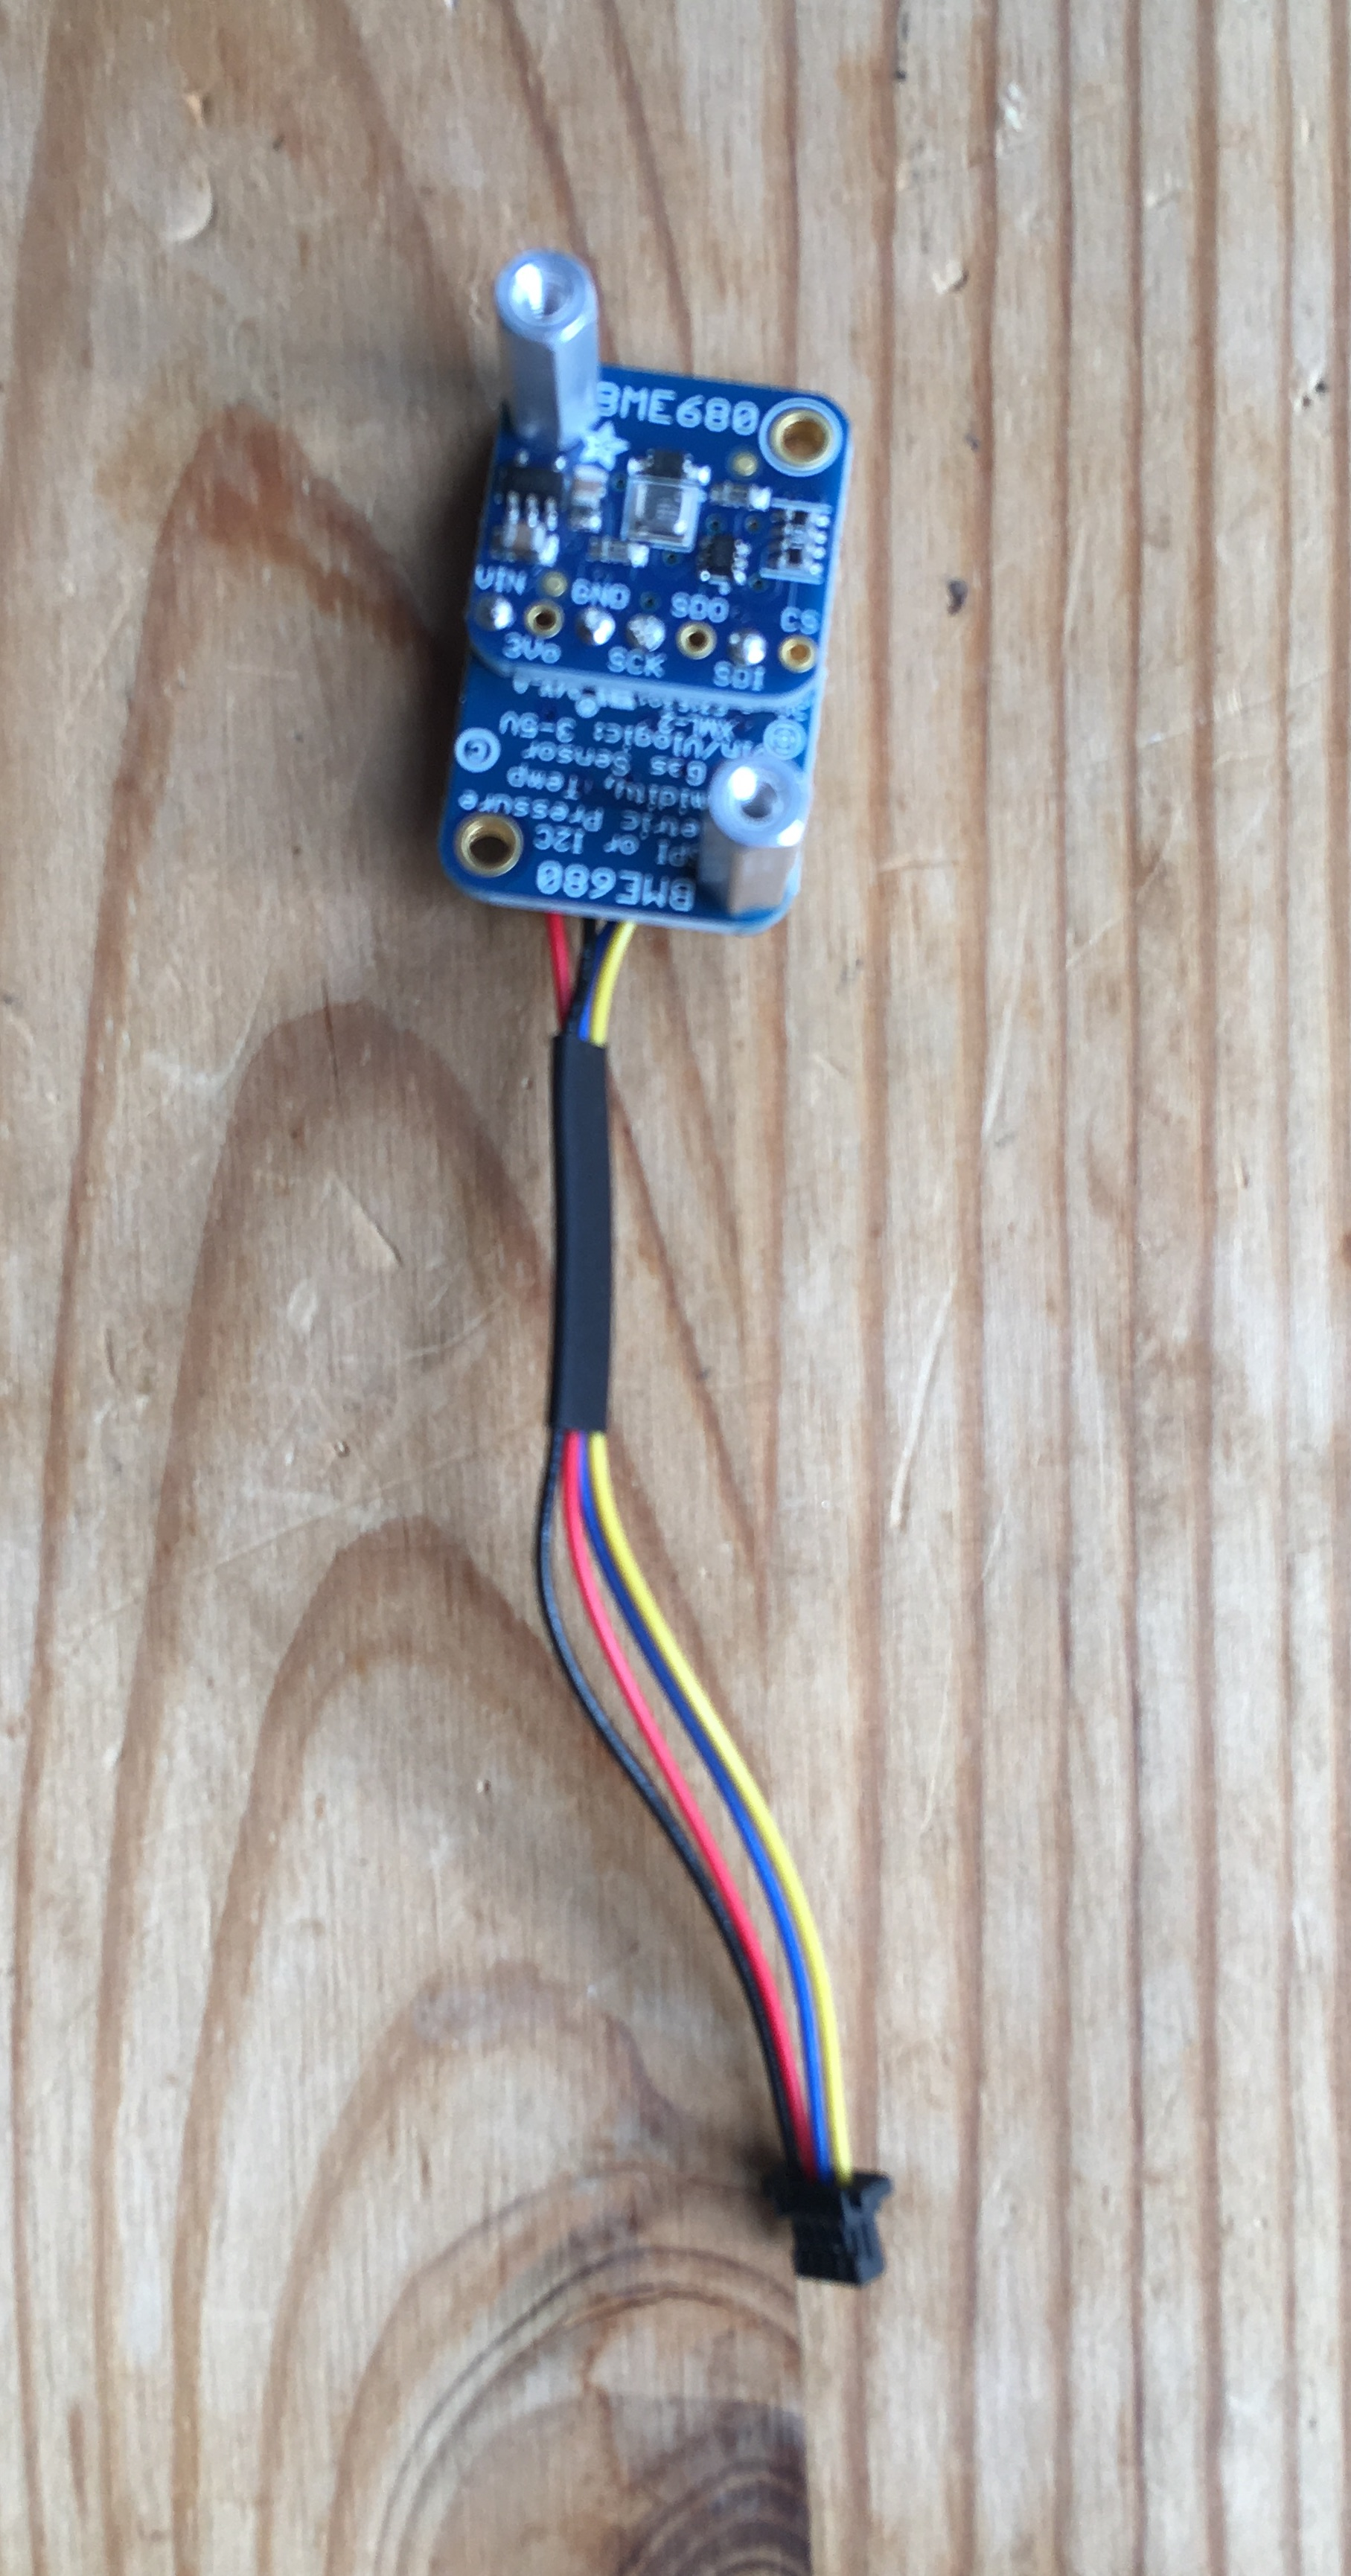
\includegraphics[width=0.4\textwidth]{images/bme_standoffs.JPG}
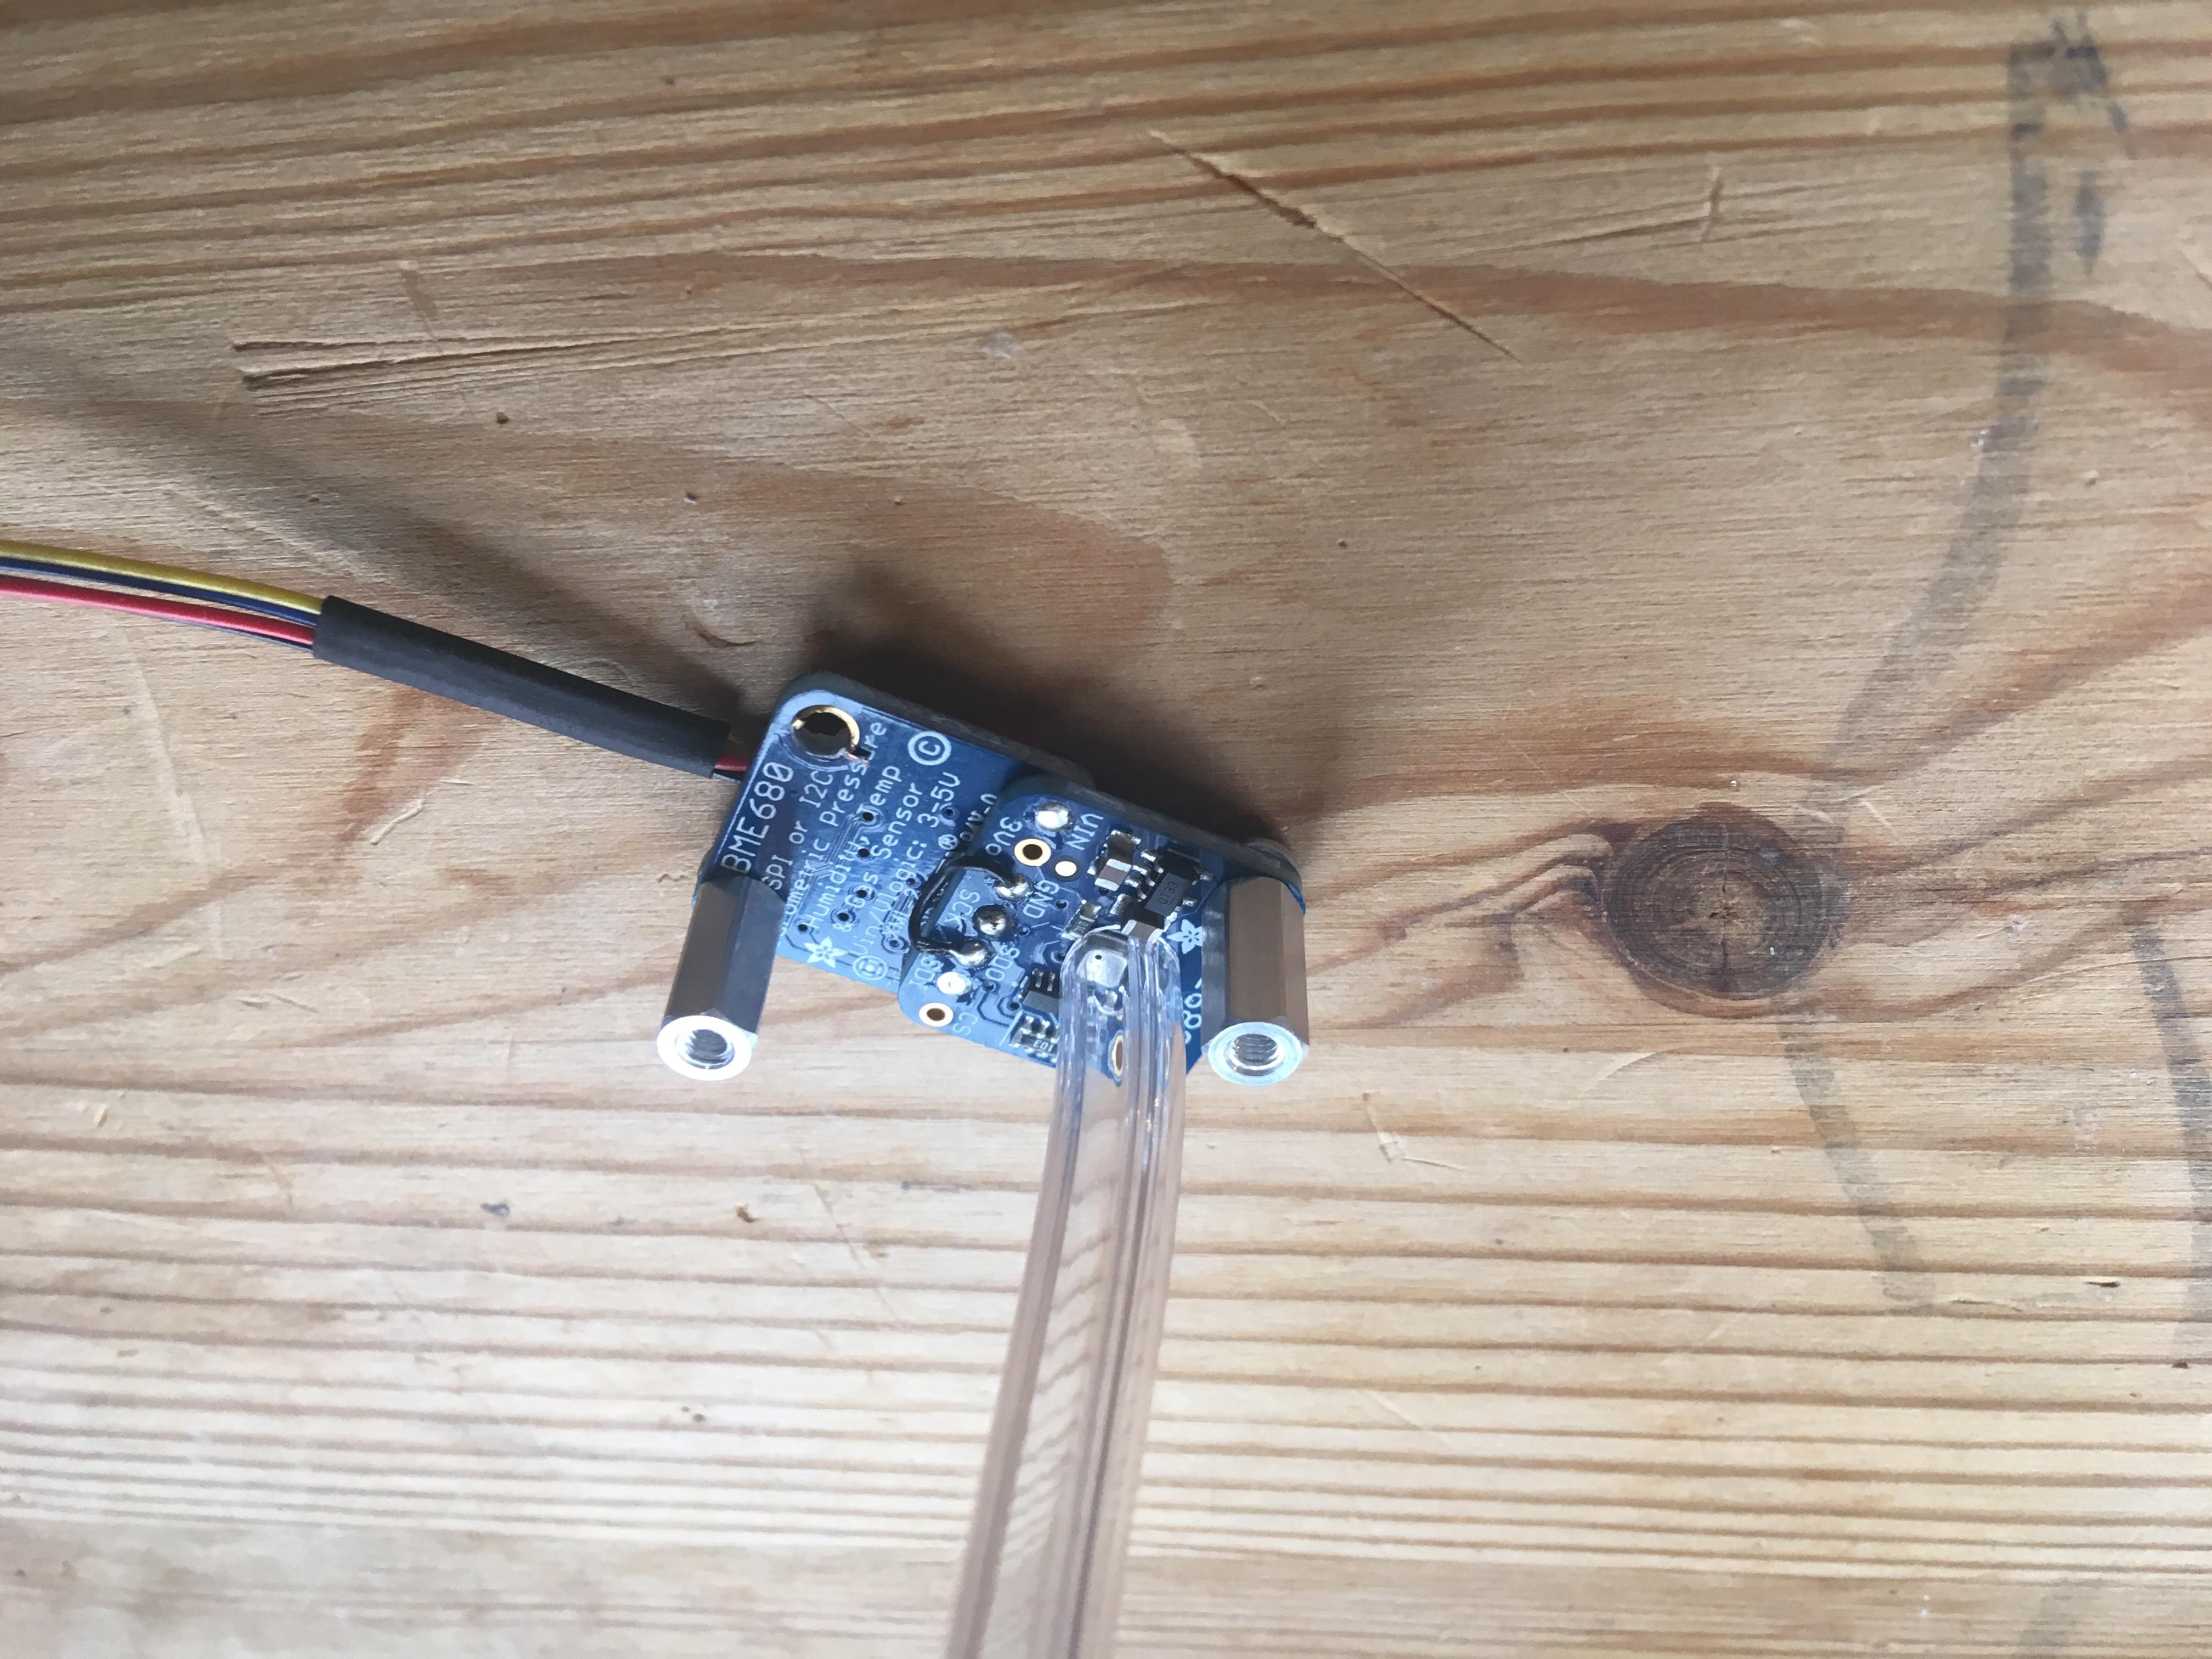
\includegraphics[width=0.6\textwidth, angle =90 ]{images/hotglue.JPG} 
\caption{Standoffs installed on pressure sensor assembly and oxygen hose prepared for gluing.} 
\label{fig:bme_glue}
\end{figure}

\item
Install pressure sensor assembly. Refer to figure \ref{fig:bmeinbox} on page \pageref{fig:bmeinbox}.
\begin{enumerate}[label=5.2.\arabic*]
\item
Add two standoffs to opposite corners of the pressure sensor assembly
\item
These should correspond to the mounting holes you drilled in the enclosure
\item
Thread the bare end of the oxygen hose through its hole in the enclose from the inside until the sensor assembly is pressed against the wall of the  enclosure
\item
Attach the standoffs into the enclosure from the outside using two machine screws
\end{enumerate}
\begin{figure}[H]
\centering
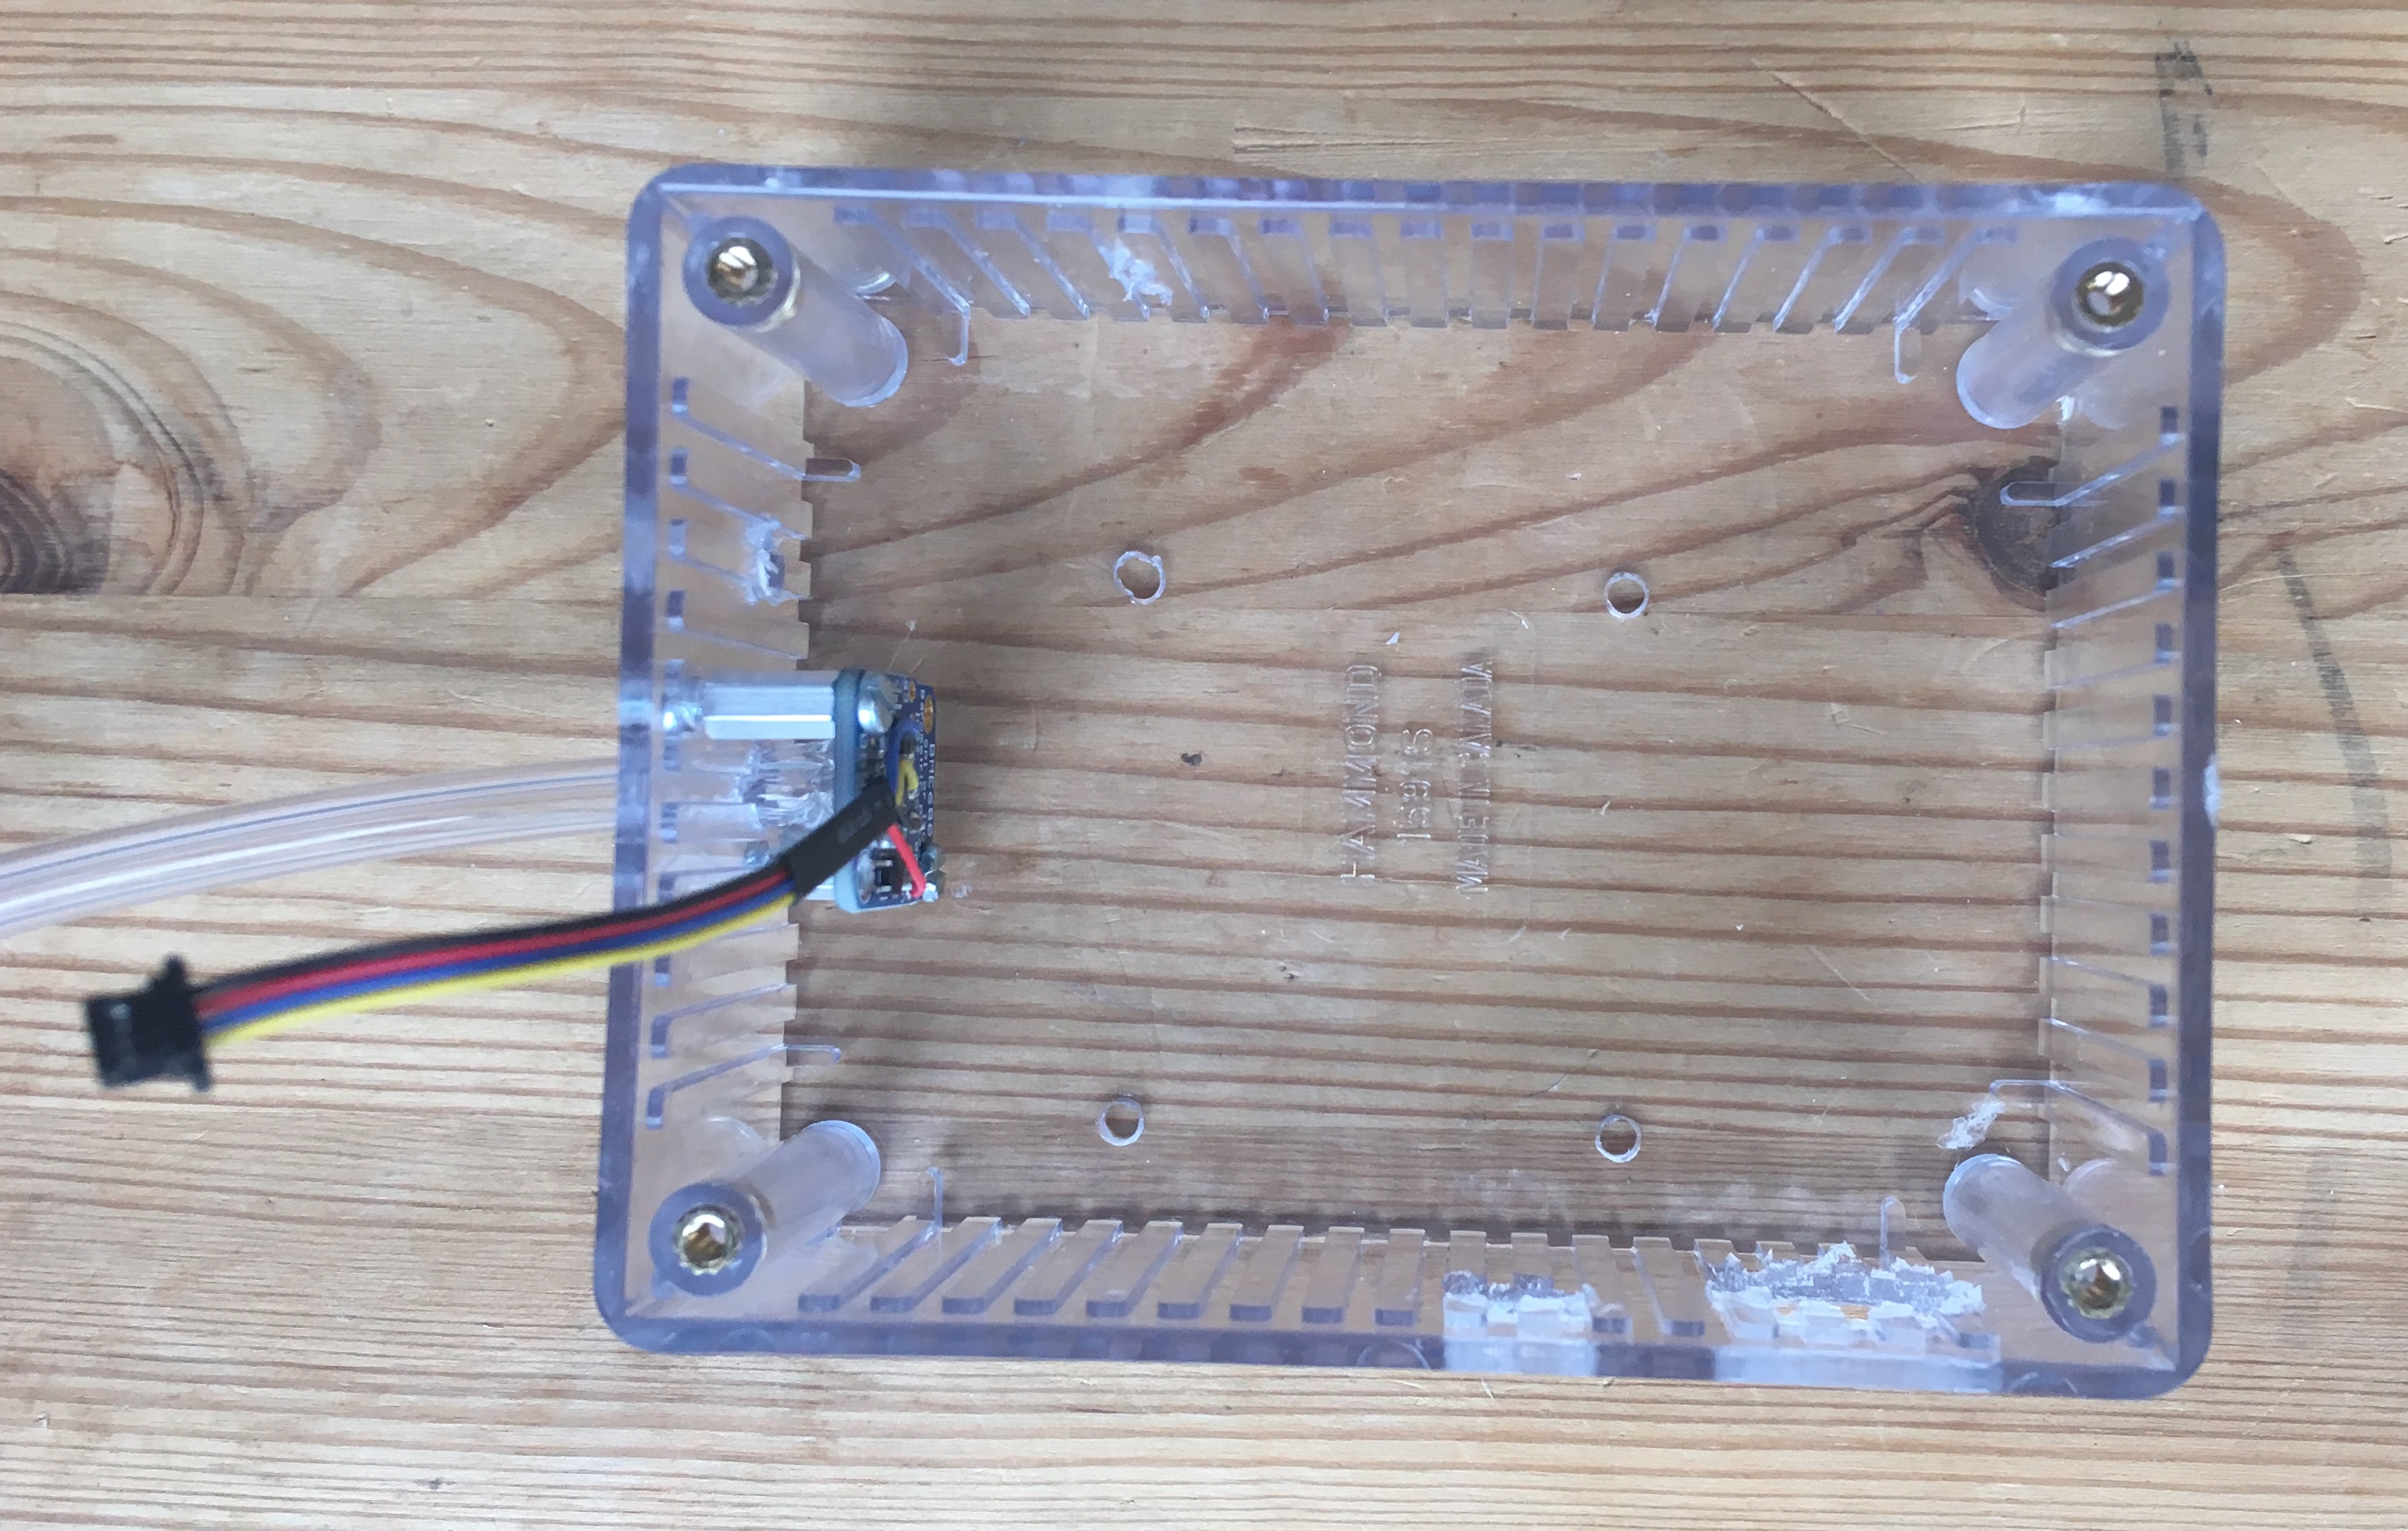
\includegraphics[width=0.8\textwidth]{images/bmeinbox.JPG} 
\caption{Pressure sensor assembly installed in enclosure.} 
\label{fig:bmeinbox}
\end{figure}
\item
Zip tie sensor cable to enclosure. Refer to figure \ref{fig:ziptie} on page \pageref{fig:ziptie}.
\begin{enumerate}[label=5.3.\arabic*]
\item
Thread the small zip tie through the two mounting holes in the enclosure
\item
Push the qwiic connector end of the flow sensor cable through its hole in the enclosure. It's a tight fit.
\item
Zip tie the cable to the side of the enclosure making sure that the jacket of the USB cable is engaged by the zip tie
\end{enumerate}
\begin{figure}[H]
\centering
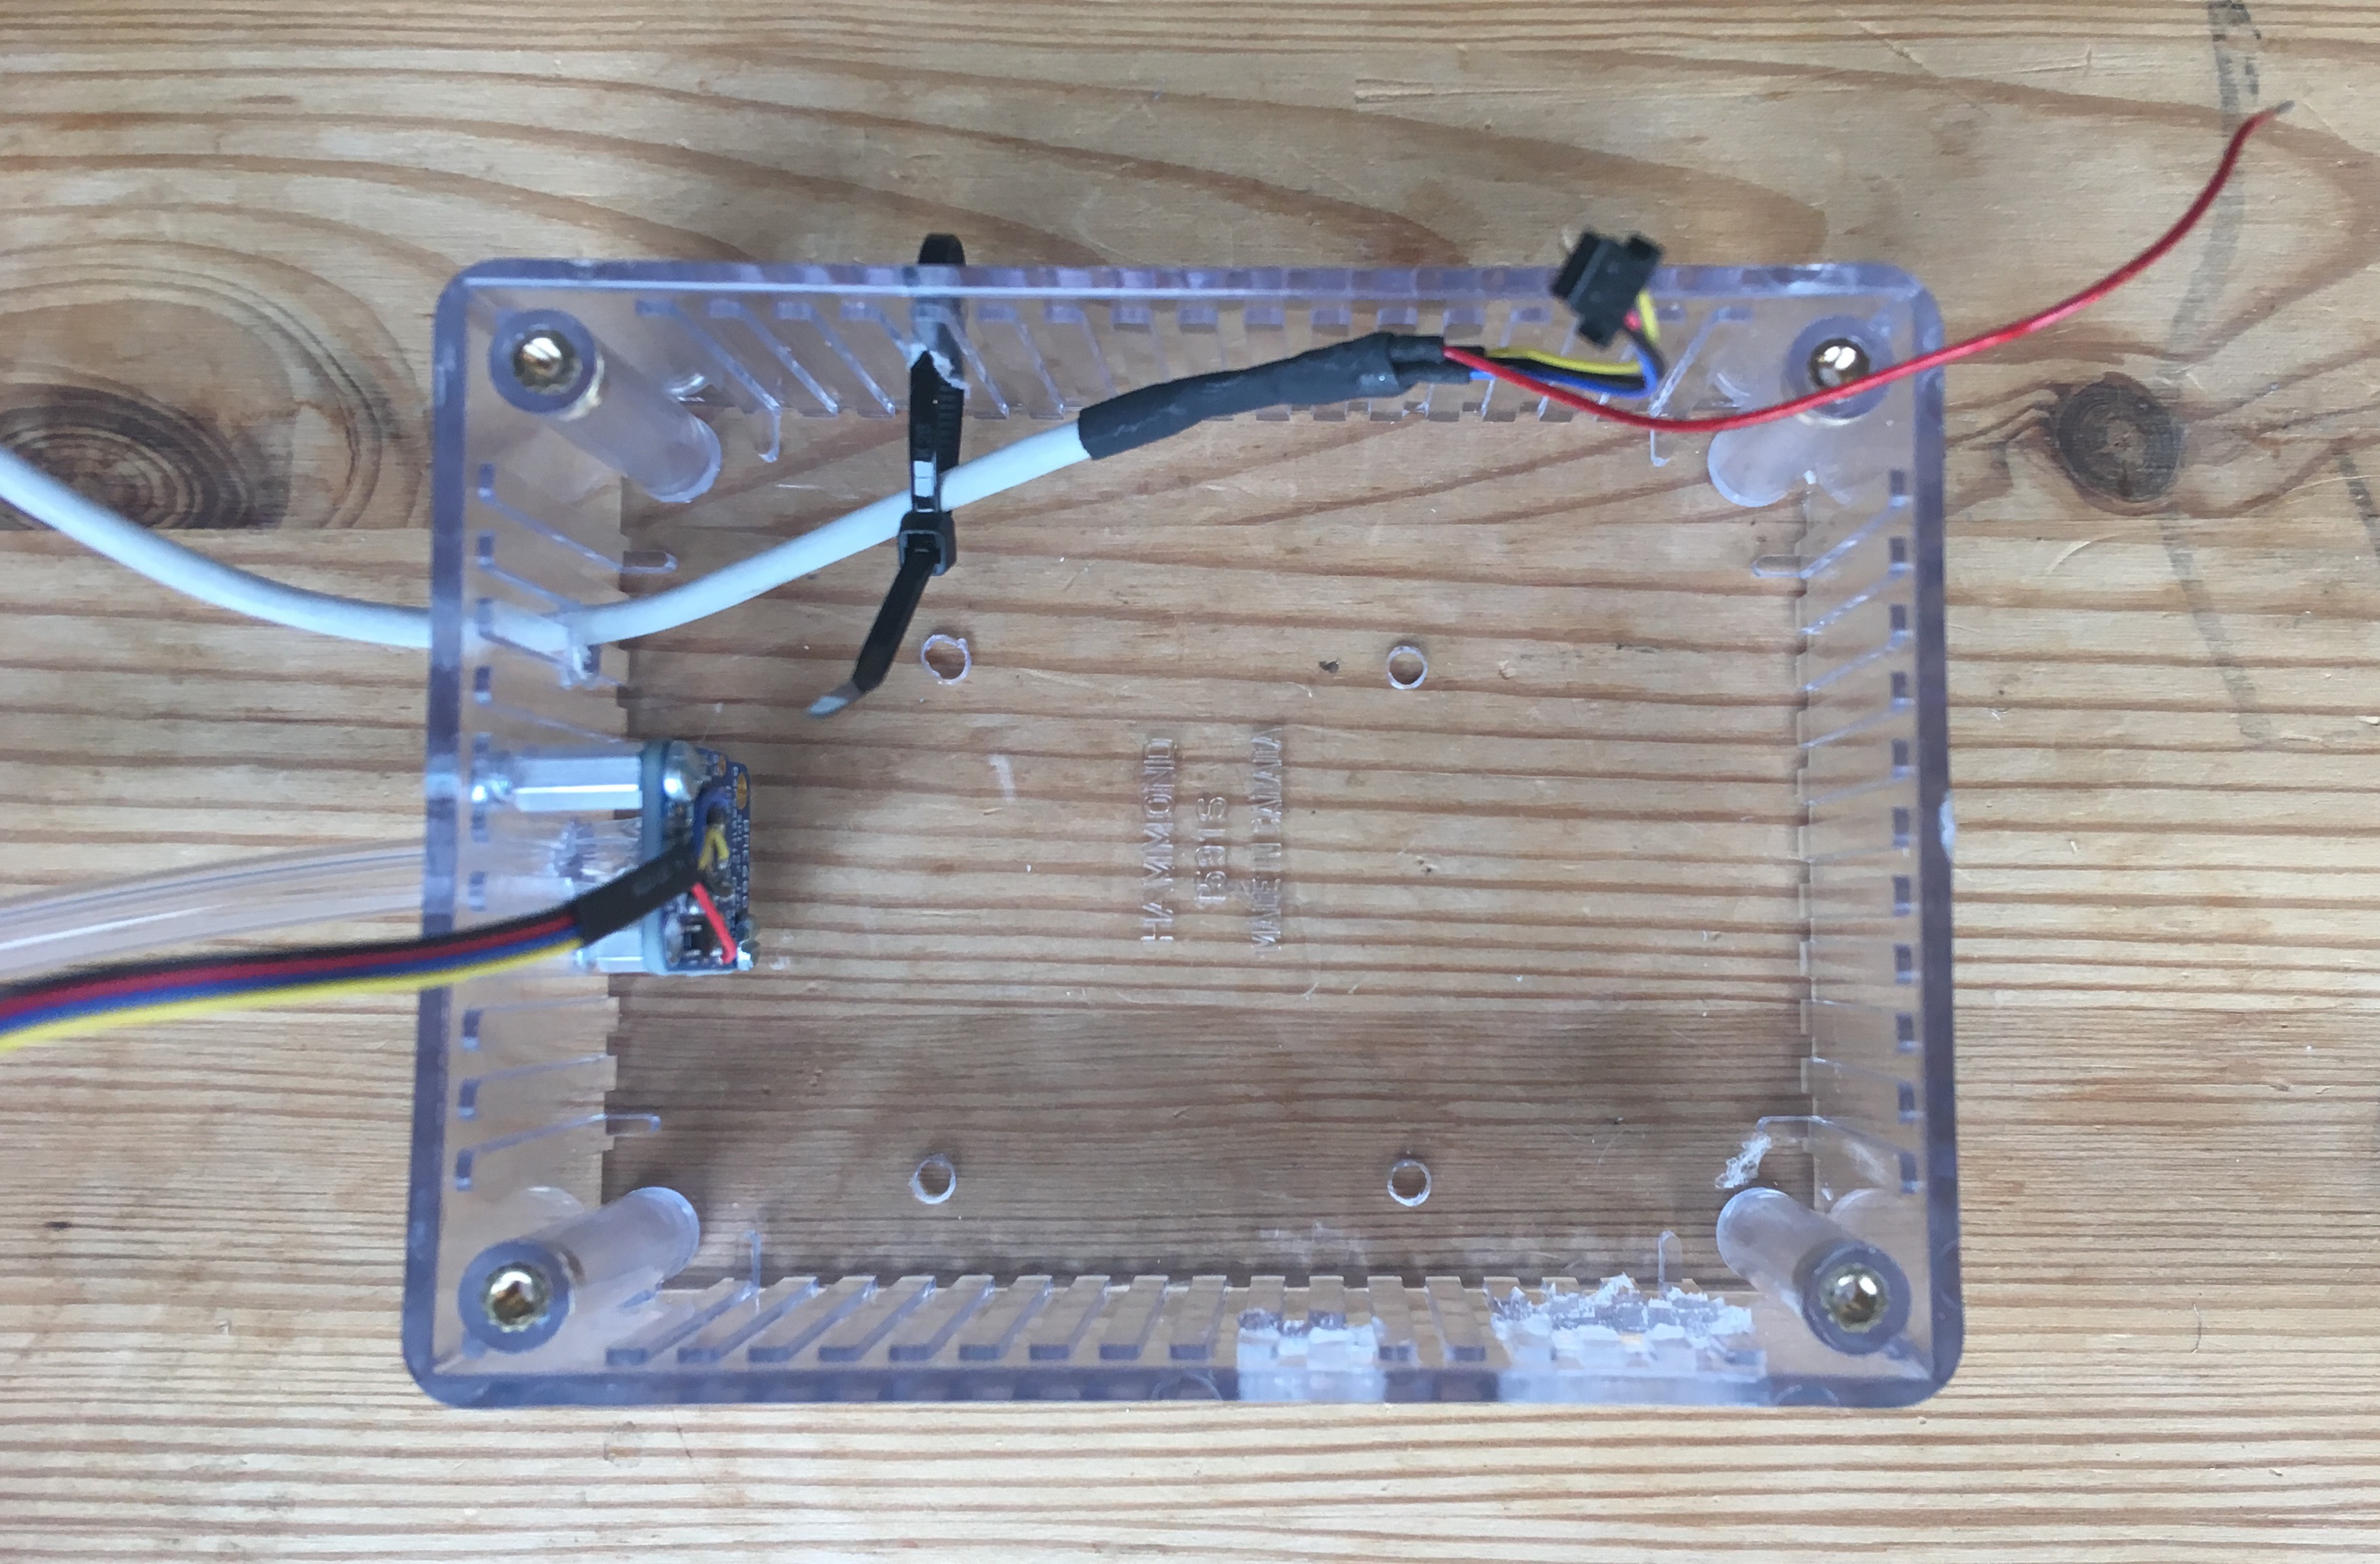
\includegraphics[width=0.8\textwidth]{images/ziptie.JPG} 
\caption{Flow sensor cable with strain relief.} 
\label{fig:ziptie}
\end{figure}


\item
Install ethernet shield and processor and add final touches.  Refer to figure \ref{fig:ziptie} on page \pageref{fig:ziptie}.
\begin{enumerate}[label=5.4.\arabic*]
\item
Attach standoffs to the four corners of the ethernet shield
\item
Screw the standoffs into the enclosure from the bottom
\item
Place the ESP32, OLED wing, and Qwiic shield on top of the ethernet shield as depicted in the diagram
\item
Plug the flow sensor and pressure sensor assembly into the qwiic shield
\item
Add a small piece of electrical tape every 5 inches attaching the oxygen tubing and flow sensor cable
\item
Wrap a piece of electrical tape around the flow sensor covering the exposed pads of the flow sensor
\item
Add identification card on the next page card to enclosure.
\begin{figure}[H]
\centering
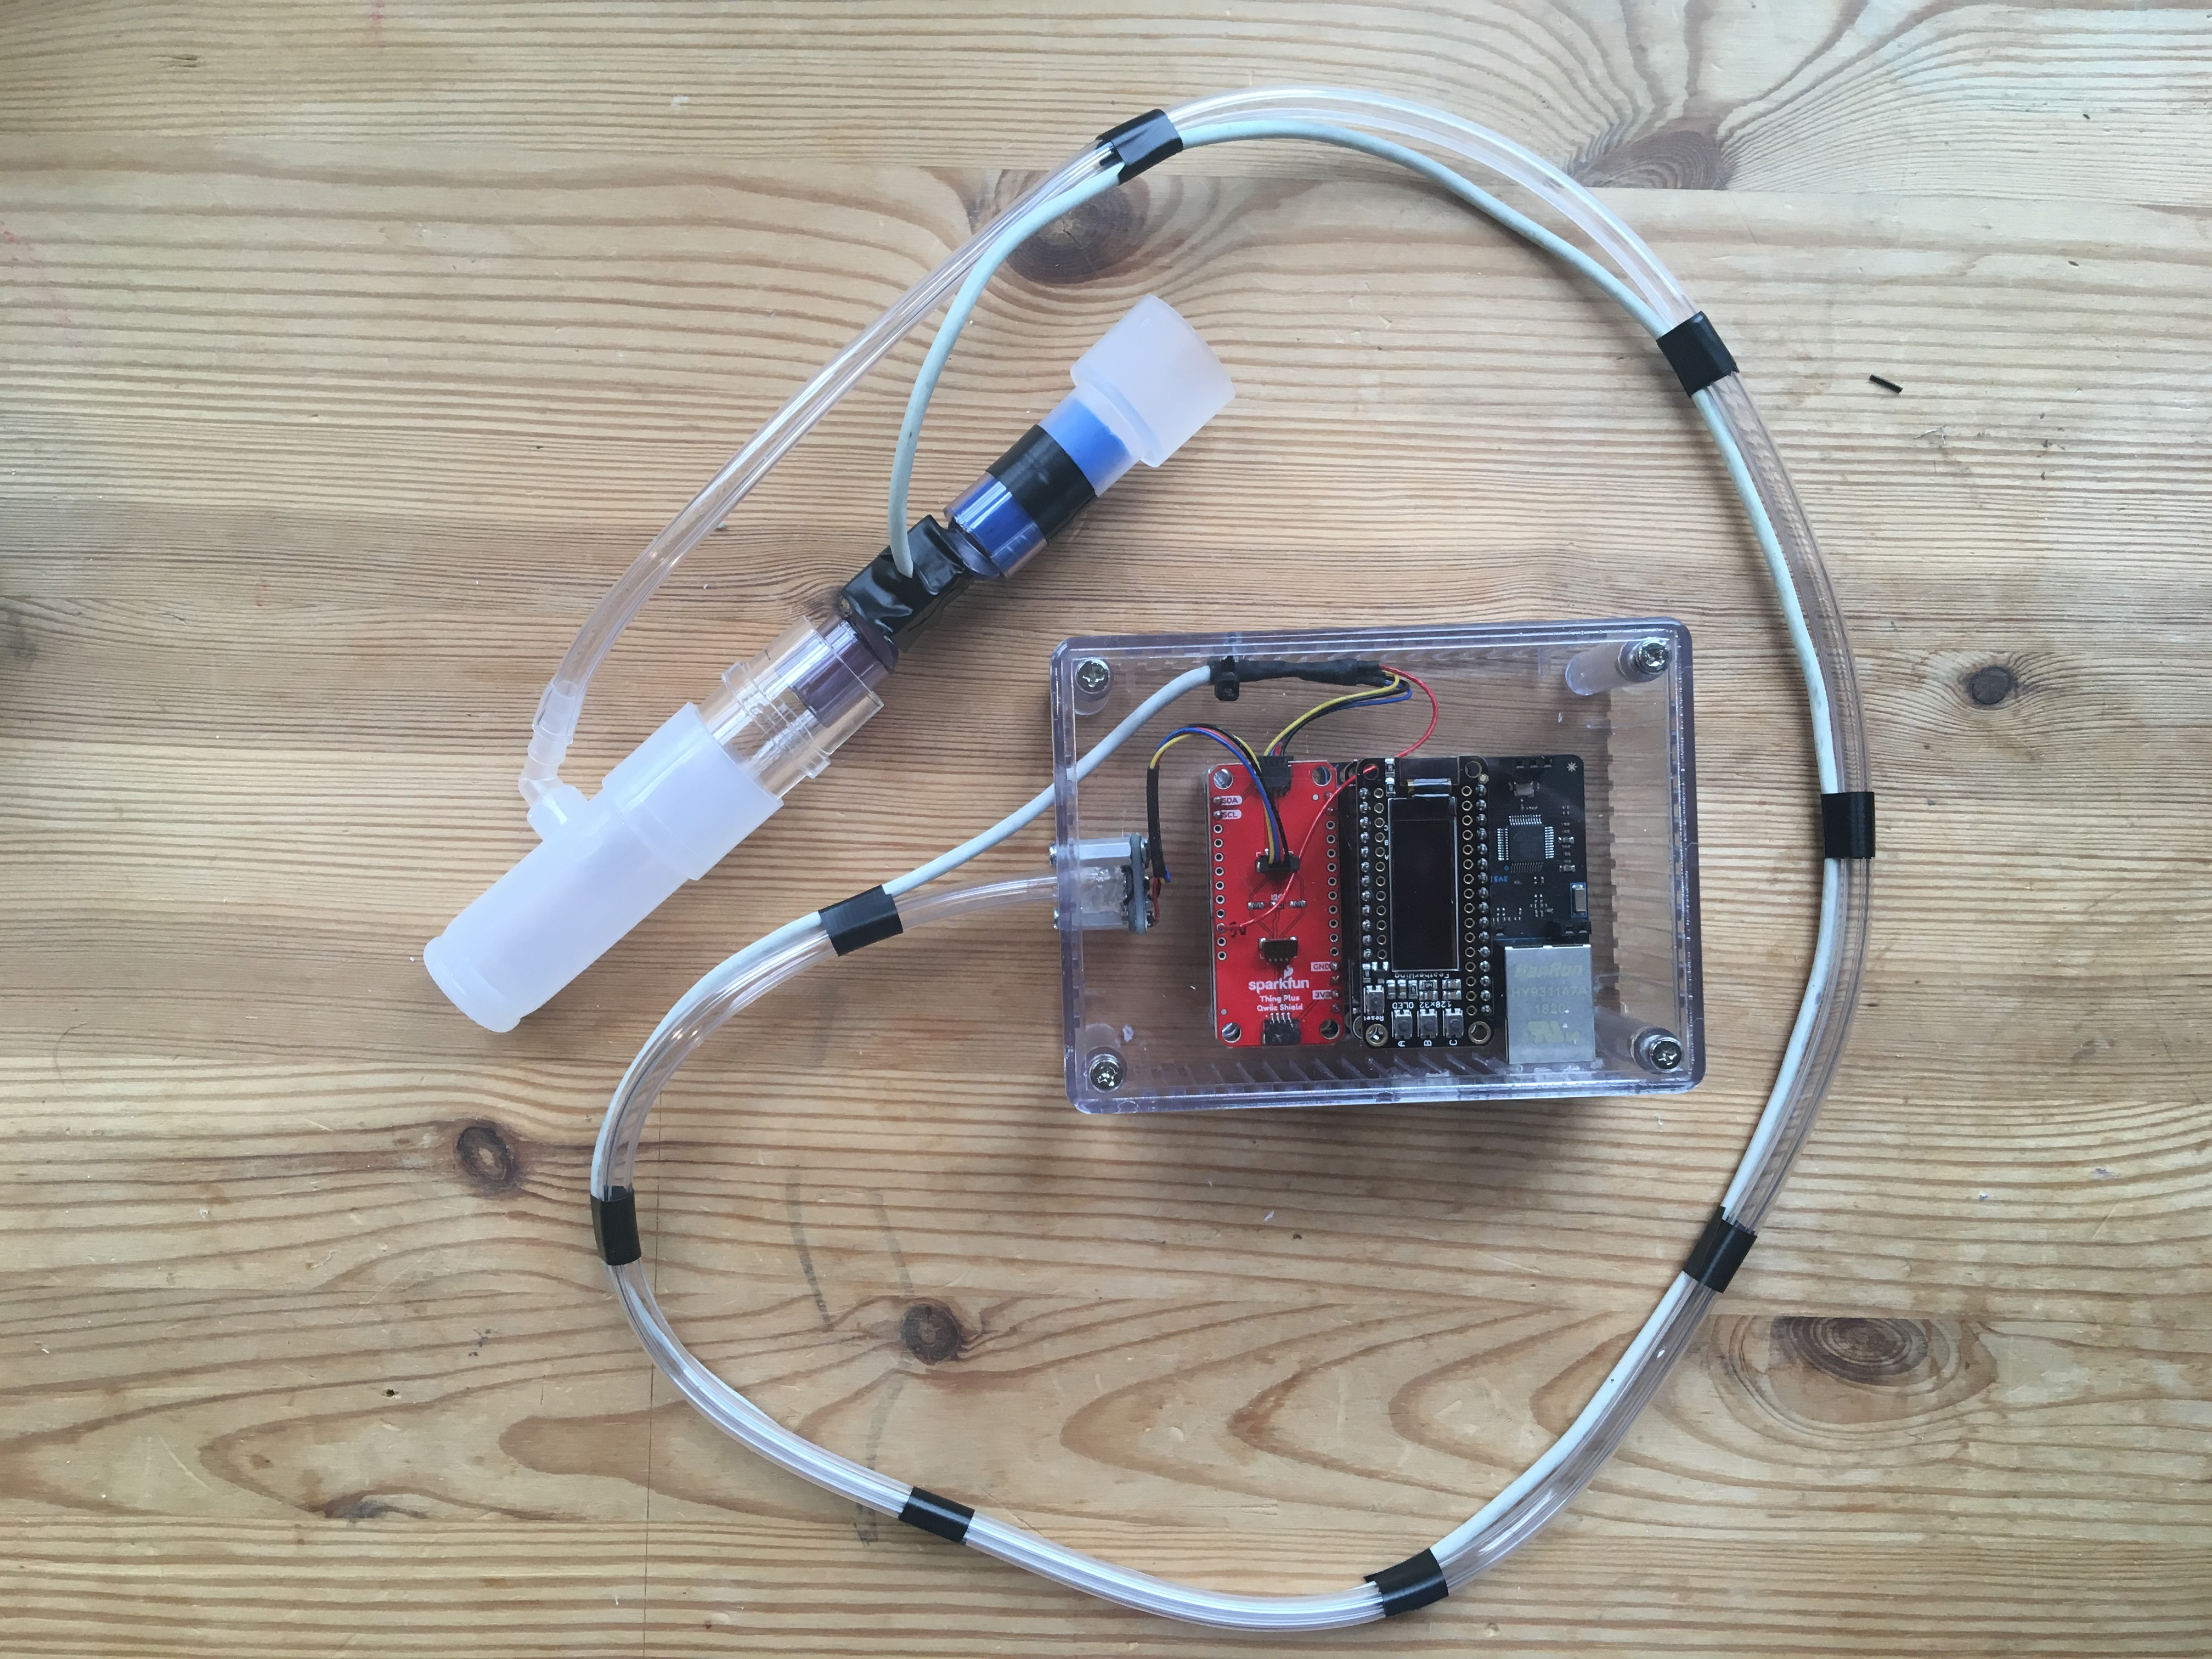
\includegraphics[width=\textwidth]{images/final_assembly_with_tape.JPG} 
\caption{Final assembly.} 
\label{fig:final}
\end{figure}
%\begin{enumerate}[label=5.4.\arabic*]
\end{enumerate}
\end{enumerate}
\end{enumerate}

%-----------------------------------------------------------

\subsection{PCB Based VentMon}

This version of VentMon requires two 3D printed parts  -- one encapsulated an on-board pressure sensor and one is an airway adaptor -- as well as a PCB assembly. Before beginning the assembly process make sure that you have manufactured those three parts.

\begin{enumerate}
\item
PCB Assembly

\begin{enumerate}[label=1.\arabic*]
\item Add standoffs to PCB
\begin{enumerate}[label=1.1.\arabic*]
\item take hardware and put it in the holes
\end{enumerate}

\item Mount sensor enclosure for BME280 pressure sensor
\begin{enumerate}[label=1.2.\arabic*]
\item Insert plastic part into mounting holes on PCB to check fit and alignment. The barb should face toward the outer edge of the PCB.
\item Apply glue to bottom edge and mounting pegs of plastic.
\item Insert plastic back into holes being careful not to get any glue on the sensor.
\item Allow 24 hours for glue to cure before attaching a hose to the barb.
\end{enumerate}


\end{enumerate}



\item
Enclosure

Follow assembly instructions in section \ref{itm:enclosure}.


\item
Flow Sensor Assembly

Follow assembly instructions in section \ref{itm:flow}.

\item
Oxygen Sensor Assembly

\begin{enumerate}[label=4.\arabic*]
\item
Screw the airflow flange on to the oxygen sensor
\item
Plug sensor into the blue airway adaptor piece
\item
Plug one end of mono audio cable into bottom of oxygen sensor
\item
Plug the other end into the audio connector on the PCB
\end{enumerate}








\item
Final Assembly

\end{enumerate}

%----------------------------------------------------------

\section{Operation instructions}
%Provide detailed instructions for the safe and proper operation of the hardware.
%> Step-by-step operational instructions for operating the hardware.
%> Use visual instructions as necessary.
%> Highlight potential safety hazards.

\textit{Provide detailed instructions for the safe and proper operation of the hardware.
\begin{itemize}
\item Step-by-step operational instructions for operating the hardware.
\item Use visual instructions as necessary.
\item Highlight potential safety hazards.
\end{itemize}}

\section{Validation and characterization}


%Demonstrate the operation of the hardware and characterize its performance over relevant critical metrics
%> Demonstrate the use of the hardware for a relevant use case.
%> If possible, characterize performance of the hardware over operational parameters.
%> Create a bulleted list that describes the capabilities (and limitations) of the hardware. For example consider descriptions of load, operation time, spin speed, coefficient of variation, accuracy, precision and etc.

Because the VentMon produces pressure and flow graphs at about 25 samples per seconds which is fast compared to
the physiological process of breathing, it is easy to have confidence in the basic dynamic function of the VentMon
by simply breathing through it into a plastic test lung. One can easily see that flow and pressure dynamically
match the breath or changes in the mechanical ventilation, or even changes induces by changes in the resistance of
compliance of the test lung.

The flow and pressure sensors used in the VentMon require not calibration. Flow was checked with a graduated syringe and
found to be quite accurate. Pressure sensors can be double checked by checking ambient pressure and, for example, computing
altitude of the physcial location.

Other aspects of ventilation such as respiration rate, peak inspiratory pressure, Inhalation to Exhalation ratio,
work of breathing, etc. are dependenent on the VentDisplay software which are a module not technically part of the VentMon
hardware. This software has been shown to be valuable, although it is dependent on accurate software decisions about
the beginning and the ending of a breath, which can be subtle in some situations.



\section{Acknowledgements}
% [List here those individuals who provided help during the research (e.g., providing language help, writing assistance or proof reading the article, etc.).] Please also identify who provided financial support for the conduct of the research and/or preparation of the article and to briefly describe the role of the sponsor(s), if any, in study design; in the collection, analysis and interpretation of data; in the writing of the report; and in the decision to submit the article for publication. If the funding source(s) had no such involvement then this should be stated.}

Robert L. Read conceived of and wrote most of the firmware for the VentMon. Geoff Mulligan created the initial cloud-based
IoT appoach which became the PIRDS-logger.
Lauria Clarke did most of the hardware design, including the assembly instructions and the printed circuit board based on an
open source design from Adafruit\cite[],
and the SFM3X00 software repo
for encapsulating Sensirion flow sensors in the Arduino environment. This paper was written by Robert L. Read and Lauria Clarke.

The Mozilla Open Source Software foundation gave Public Invention a grant that allowed us to develop the hardware and
provide 20 VentMons to open source teams around the world free-of-charge, including paying shipping costs.
Protocol Labs provided Public Invention a grant that has been used web communication and conference costs.

We would like to thank early adopters of the VentMon on pandemic ventilator teams such as the ARMEE\cite{} and
DIY-Beatmungsgerät.de\cite{}
who gave us valuable bug reports and feedback.

Student volunteers on the COVID19-vent-list project\cite{} helped to make the need for the VentMon clear by assessing over 100
pandemic ventilator teams.

\section{Declaration of interest}

None.
% a statement must be included even if there is no conflict of interest
% All authors must disclose any financial and personal relationships with other people or organizations that could inappropriately influence (bias) their work. Examples of potential conflicts of interest include employment, consultancies, stock ownership, honoraria, paid expert testimony, patent applications/registrations, and grants or other funding. Authors must disclose any interests in a summary declaration of interest statement in the manuscript file. If there are no interests to declare then please state this: 'Declarations of interest: none'. This summary statement will be ultimately published if the article is accepted. More information.}



% This work touched no humans or animals, I belive this section can be ommmited entirely.
% \section{Human and animal rights}

\iffalse

\section*{References}
%> Include at least one reference, to the original publication of the hardware you customized.
%> Include other references as required. Include references to put your device in context in the literature. For more information on the reference format in HardwareX please see the Guide for Authors at: https://www.elsevier.com/journals/hardwarex/2468-0672/guide-for-authors

\textit{\begin{itemize}
\item Include at least one reference, to the original publication of the hardware you customized.
\item Include other references as required. Include references to put your device in context in the literature. For more information on the reference format in HardwareX please see the Guide for Authors at: https://www.elsevier.com/journals/hardwarex/2468-0672/guide-for-authors
\end{itemize}}


\fi

\end{document}

%> Author manuscript checklist
%> ●	HardwareX is a journal dedicated to the exhaustive and fully open source communication of advances in scientific infrastructure. Upon submission the author declares that all information necessary to reproduce the subject of the submission (e.g. bill of materials, build instructions, calibration procedures, source files, code, and safety considerations) is communicated in full and is accessible for use under an open source license.
%> ●	Is the subject of the submission under an open source license - as defined by the Open Source Hardware definition?
%> ●	Can the hardware be reproduced with the details provided in the submission?
%> ●	Are all relevant design files available on Mendeley Data, the Open Science Framework, or Zenodo repositories, described in the Summary of Design Files document, and clearly documented? (e.g. descriptive file names, commented code, labeled images, etc.)
%>      ○	If in the Open Science Framework, the repository has be registered? Instructions
%>      ○	If in Zenodo, the repository is open access and is published? Instructions
%>      ○	If in Mendeley Data, the repository is published or the sharable link was included in the additional information of the Editorial Submission interface? Instructions
%> ●	Are visual instructions used when necessary?
%> ●	Is the utility of the hardware to the scientific community?
%> ●	Is the performance of the hardware adequately demonstrated and characterized?
%> ●	Are all potential safety concerns addressed?
%> ●	For more information on the article template consult the Guide to Authors.}


% Notes:
% Potential reviewers: Michelle Mellenthin, Eric Schulz

% Here is our BibTex entry to the DOI for this version:
@software{robert_l_read_2020_4079170,
  author       = {Robert L. Read and
                  Lauria Clarke and
                  Darío Hereñú and
                  Geoff Mulligan},
  title        = {{PubInv/ventmon-ventilator-inline-test-monitor:
                   v0.3T - Ventmon Tester 0.3}},
  month        = oct,
  year         = 2020,
  publisher    = {Zenodo},
  version      = {v0.3T},
  doi          = {10.5281/zenodo.4079170},
  url          = {https://doi.org/10.5281/zenodo.4079170}
}

@misc{
  author = {Robert L. Read and
    Avinash Baskaran and
    Enrique Villacres and
    Keeshan Patel},
  title = {COVID-19 Vent List},
  month        = oct,
  year         = 2020,
  url = {https://docs.google.com/spreadsheets/d/1inYw5H4RiL0AC_J9vPWzJxXCdlkMLPBRdPgEVKF8DZw/edit#gid=0}
  }

@mics{ARMEE,
  url = {https://armeevent.com/}
}
@misc{beatmnug,
  url = {https://www.xn--diy-beatmungsgert-5qb.de/}
  }
